\chapter{Mathematical Representations of Uncertainty}

\section{Notations}
We introduce here a few notations that will be used in the rest of this chapter. \comroman{A ajouter au fur et à mesure}
\begin{itemize}
    \item \st means ``such that''
    \item We will often present theorems or results with $n$ different variables, spaces, or Cartesian products of $n$ elements. Notations therefore quickly become quite heavy. We try our best to make them clear and readable, which is why we often use the contraction ``$\dots$'' to imply that we are enumerating all variables. For instance, if we apply a function $f$ to four variables $x_1, x_2, x_3, x_4$, we will write $f(x_1, \dots, x_4)$.
    \item When working with $n$ variables, the index $i$ will usually be used to refer to the $i$-th variable (or one of its attribute), and will be appended as a subscript when possible, otherwise as a superscript. For instance, if $x\in\mathbb{R}^n$, then $x_i$ will refer to the $i$-th component of $x$. If $m_\times\in\mathbb{R}^n$, then $m_\times^i$ will refer to $i$-th component of $m_\times$.
    \item $\opi\cdot,\cdot\cli$ refers to an interval of integers. For instance $\opi1,~4\cli=\{1,~2,~3,~4\}$. 
    \item CDF will refer to Cumulative Distribution Function, \ie if $X$ is random variable in $\mathbb{R}$ and $P$ its associated probability, then the CDF of $X$ is $F(x)=P(X\leqslant x)$.
    \item The power set of a set $\X$ is noted $2^\X$. It correspond to the set of all sets included in $\X$. In the discrete case, if the cardinal of $\X$ is $n$, then the cardinal of the power set is $2^n$, thus the notation.
\end{itemize}


\comseb{Ca ne me semble pas forcément idéal de faire du spécifique $->$ général $->$ spécifique? Dans un sens, les possibilités qui étendent les ensembles sont tout aussi "fondamentale" que les probabilités. Introduire d'abord l'idée générale de modèle d'incertitude, puis décliner les modèles particulier dont tu auras besoin?}

\section{Probabilities}
Define what is an atom
Classical framework to represent uncertainty. Epistemic vs stochastic uncertainty. Paradoxes with uniform distribution, dependency (sum of dices etc). Definition of a random variable \etc
\section{Gambles, imprecise probabilities}
Introduction to IP, how it contains the classical probability framework. Pboxes there?
Define coherence, sure loss, cylindrical sets
\section{Specific case of possibility distributions}
Link with fuzzy sets. A simple and useful model, but with limited expressiveness (n focal sets and not $2^n$). Nested focal sets. Used to model experts opinions with examples \cite{baudrit_joint_2007}

\section{Copulas}\label{sec:copulas}
\comroman{Define also sub copulas\\Talk briefly about imprecise copula too}

In the following sections, we will work with multiple random variables. Let $n\in\mathbb{N}^*$ be the number of random variables considered. A copula is a multivariate distribution function $C:[0,1]^{n}\rightarrow [0,1]$ whose marginals follow uniform distributions on $[0,1]$. It can be interpreted as a joint cumulative distribution of $n$ random variables. For all $i\in\opi 1,n\cli $, we will refer to $u_i\in[0,1]$ as its $i$-th variable (or marginal). A copula verifies a number of properties:
\begin{align}
    &\text{if }\exists j\in\opi 1,n\cli  \text{ \st }~u_j=0, \text{ then }C(u_1,\dots,u_j,\dots,u_n)=0\label{eq:zero_copula}\\
    &\forall i\in\opi 1,n\cli ,~C(1,1,\dots,1,u_i,1,\dots,1)=u_i\label{eq:copula_ones}\\
    &\forall (v_1,\dots,v_n)\in[0,1]^n \text{ \st }~\forall i\in\in\opi 1,n\cli ,~v_i\geqslant u_i\nonumber\\
    &\sum_{(w_1, \dots, w_n)\in\Pi_{i=1}^n\{u_i, v_i\}}(-1)^{|\{i~|~w_i=u_i\}|}C(w_1, \dots, w_n)\geqslant 0\label{eq:cop_hvolume}
\end{align}
where $\Pi_{i=1}^n$ is the Cartesian product of $n$ elements, meaning that $(w_1, \dots, w_n)\in\Pi_{i=1}^n\{u_i, v_i\}$ is a tuple of $n$ elements, where each element is either $u_i$ or $v_i$. Additionally, $|\{i~|~w_i=u_i\}|$ refers to the cardinal of the set $\{i~|~w_i=u_i\}$. The first term in equation \eqref{eq:cop_hvolume} is also called H-volume or hyper-volume. It is used to compute joint probability mass assignments in the precise case (and also in the imprecise case, see section \ref{sec:joint_mass}). In the rest of this thesis, we will use the following notation to refer to the $H$-volume:
\begin{eqnarray}\label{eq:hvolume}
    &&\forall i\in\opi 1,n\cli ,~\forall~0\leqslant u_i \leqslant v_i \leqslant 1,\nonumber\\
    &&H^{v_1,\dots v_n}_{u_1,\dots,u_n}=\sum_{(w_1, \dots, w_n)\in\Pi_{i=1}^n\{u_i, v_i\}}(-1)^{|\{i~|~w_i=u_i\}|}C(w_1, \dots, w_n)
\end{eqnarray}
The formula of the H-volume can be difficult to grasp in the general case. A way of interpreting it is presented later after theorem \ref{theorem:sklar}.

A central theorem regarding copulas is Sklar's theorem \cite{sklar_fonctions_1959}:
\begin{theorem}[Sklar's theorem]\label{theorem:sklar}
    Let $F:\X_1\tdt\X_n\rightarrow[0,1]$ be a multivariate cumulative distribution function, where $\X_i\subseteq\overline{\mathbb{R}}$. The marginals $F_i$ of $F$ are defined as $\forall i\in\opi 1,n\cli , \forall x\in\X_i, F_i(x) = F( +\infty, \dots,  +\infty, x,  +\infty, \dots, +\infty)$ where $x$ is the $i$-th component of $F$. If $F_i$ are continuous, then a unique copula $C$ exists on $\X_1\tdt\X_n$ such that:
    \begin{eqnarray}
        \forall (x_1,\dots,x_n)\in \overline{\mathbb{R}}^n, F(x_1,\dots,x_n)=C(F_1(x_1),\dots, F_n(x_n))
    \end{eqnarray}
    If $F_i$ are not continuous, then $C$ is unique on the product of the ranges of $F_i$.
    The reverse is also true: any copula applied to univariate cumulative distribution functions yields a multivariate cumulative distribution function whose marginals are the univariate CDFs.
\end{theorem}

It follows from \eqref{eq:cop_hvolume} that a copula is a component-wise increasing mapping. All copulas are dominating and dominated by two bounds (called lower and upper Fréchet–Hoeffding)
\begin{align}
    &\forall u_i \in [0,1]^n,\nonumber\\
    &\max(0, 1-n+\sum_{i=1}^n u_i) \leqslant C(u_1,\dots,u_n) \leqslant \min(u_1, \dots, u_n)
\end{align}
The upper bound is a copula, usually called the Minimum copula $C_M$, modelling co-monotonic variables. The lower bound is a copula only in the case $n=2$, called the \L ukasiewicz copula $C_L$, modelling counter-monotonic variables. However, for every $u_1,\dots,u_n$, there exists a copula attaining the lower bound:
\begin{eqnarray*}
    \forall (u_1,\dots,u_n)\in[0,1]^n,~\exists C \text{ \st }~C(u_1,\dots,u_n) = \max(0, 1-n+\sum_{i=1}^n u_i)
\end{eqnarray*}

Independence between variables is modeled by the product copula $C_\Pi(u_1, \dots, u_n)=u_1\dots u_n$, which will be used later in subsection \ref{subsection:product_copula}. Graphical representations of the product copula and of the lower and upper Fréchet–Hoeffding bounds are represented in figure \ref{fig:copulas}. Some examples of families of copulas that can be generated using a single parameter $\theta$ in the case $n=2$ are presented in table \ref{tab:familiy_of_copula}. Another important family of copulas is the family of Gaussian copulas. Each Gaussian copula is generated with a correlation matrix $R\in[-1,1]^{(n,n)}$:
\begin{align}
    C_R=\Phi_R(\Phi^{-1}(u_1), \dots, \Phi^{-1}(u_n)) \label{eq:gaussian_copula}
\end{align} where $\Phi_R$ is the joint multivariate cumulative distribution function of a Gaussian variable with correlation matrix $R$, and $\Phi^{-1}$ is the inverse cumulative distribution function of a univariate Gaussian variable. 

\begin{figure}
    \centering
        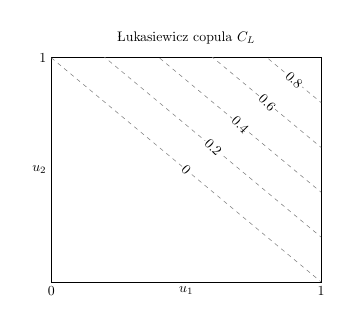
\begin{tikzpicture}[scale=0.5]
        \begin{axis}[
            xmin=0,xmax=1,
            ymin=0,ymax=1,
            xtick={0, 0.5, 1},
		    xticklabels={$0$, $u_1$, $1$},
		    ytick={0.5, 1},
		    yticklabels={$u_2$, $1$},
		    xtick style={draw=none},
		    ytick style={draw=none},
            title={\L ukasiewicz copula $C_L$},
            ]
            \addplot [domain=0:1,samples=40,style=dashed,color=gray]({x},{1-x});
            \addplot [domain=0:1,samples=40,style=dashed,color=gray]({x},{1.2-x}); 
            \addplot [domain=0:1,samples=40,style=dashed,color=gray]({x},{1.4-x}); 
            \addplot [domain=0:1,samples=40,style=dashed,color=gray]({x},{1.6-x}); 
            \addplot [domain=0:1,samples=40,style=dashed,color=gray]({x},{1.8-x});

            \node[rotate=-45, fill=white, rounded corners=2pt, inner sep=1pt] (x) at (0.5, 0.5) {0};
            \node[rotate=-45, fill=white, rounded corners=2pt, inner sep=1pt] (x) at (0.6, 0.6) {0.2};
            \node[rotate=-45, fill=white, rounded corners=2pt, inner sep=1pt] (x) at (0.7, 0.7) {0.4};
            \node[rotate=-45, fill=white, rounded corners=2pt, inner sep=1pt] (x) at (0.8, 0.8) {0.6};
            \node[rotate=-45, fill=white, rounded corners=2pt, inner sep=1pt] (x) at (0.9, 0.9) {0.8};
        \end{axis}
        \end{tikzpicture}\quad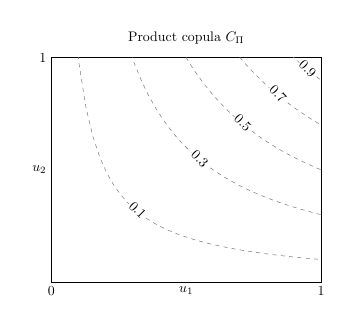
\begin{tikzpicture}[scale=0.5]
        \begin{axis}[
            xmin=0,xmax=1,
            ymin=0,ymax=1,
            xtick={0, 0.5, 1},
		    xticklabels={$0$, $u_1$, $1$},
		    ytick={0.5, 1},
		    yticklabels={$u_2$, $1$},
		    xtick style={draw=none},
		    ytick style={draw=none},
            title={Product copula $C_\Pi$},
            ]
            \addplot[domain=0:1,samples=40,style=dashed,color=gray]({x},{0.1/x});
            \addplot[domain=0:1,samples=40,style=dashed,color=gray]({x},{0.3/x}); 
            \addplot[domain=0:1,samples=40,style=dashed,color=gray]({x},{0.5/x}); 
            \addplot[domain=0:1,samples=40,style=dashed,color=gray]({x},{0.7/x}); 
            \addplot[domain=0:1,samples=40,style=dashed,color=gray]({x},{0.9/x});

            \node[rotate=-45, fill=white, rounded corners=2pt, inner sep=1pt] (x) at (0.32, 0.32) {0.1};
            \node[rotate=-45, fill=white, rounded corners=2pt, inner sep=1pt] (x) at (0.55, 0.55) {0.3};
            \node[rotate=-45, fill=white, rounded corners=2pt, inner sep=1pt] (x) at (0.71, 0.71) {0.5};
            \node[rotate=-45, fill=white, rounded corners=2pt, inner sep=1pt] (x) at (0.84, 0.84) {0.7};
            \node[rotate=-45, fill=white, rounded corners=2pt, inner sep=1pt] (x) at (0.95, 0.95) {0.9};
            
        \end{axis}
        \end{tikzpicture}\quad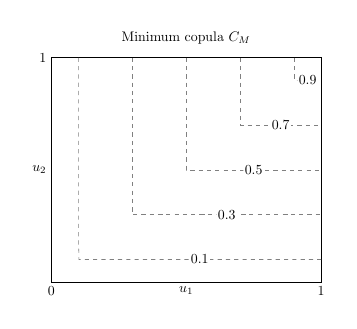
\begin{tikzpicture}[scale=0.5]
        \begin{axis}[
            xmin=0,xmax=1,
            ymin=0,ymax=1,
            xtick={0, 0.5, 1},
		    xticklabels={$0$, $u_1$, $1$},
		    ytick={0.5, 1},
		    yticklabels={$u_2$, $1$},
		    xtick style={draw=none},
		    ytick style={draw=none},
            title={Minimum copula $C_M$},
            ]
            \addplot [domain=0:1,samples=40,style=dashed,color=gray]({max(x, 0.1)},{max(1-x/0.1,0.1)});
            \addplot [domain=0:1,samples=40,style=dashed,color=gray]({max(x, 0.3)},{max(1-x/0.3,0.3)});
            \addplot [domain=0:1,samples=40,style=dashed,color=gray]({max(x, 0.5)},{max(1-x/0.5,0.5)});
            \addplot [domain=0:1,samples=40,style=dashed,color=gray]({max(x, 0.7)},{max(1-x/0.7,0.7)});
            \addplot [domain=0:1,samples=40,style=dashed,color=gray]({max(x, 0.9)},{max(1-x/0.9,0.9)});

            \node[fill=white, rounded corners=2pt, inner sep=1pt] (x) at (0.55, 0.1) {0.1};
            \node[fill=white, rounded corners=2pt, inner sep=1pt] (x) at (0.65, 0.3) {0.3};
            \node[fill=white, rounded corners=2pt, inner sep=1pt] (x) at (0.75, 0.5) {0.5};
            \node[fill=white, rounded corners=2pt, inner sep=1pt] (x) at (0.85, 0.7) {0.7};
            \node[fill=white, rounded corners=2pt, inner sep=1pt] (x) at (0.95, 0.9) {0.9};
        \end{axis}
        \end{tikzpicture}
    \caption{Bird view of the \L ukasiewicz, product and Min copulas for $n=2$. Dashed gray lines represent isolines of the copulas.}
    \label{fig:copulas}
\end{figure}


{\renewcommand{\arraystretch}{2}%
\begin{table}[!ht]
    \centering
    \begin{tabular}{|c|c|c|c|c|}
        \hline
        Family & $C(u_1,u_2)$ & $\theta$ & D-convex & D-concave \\
        \hline\hline
        Ali-Mikhail-Haq & $\frac{u_1u_2}{1-\theta(1-u_1)(1-u_2)}$ & $[-1,1)$ & $\theta\leqslant0$ & $0\leqslant\theta$ \\
        \hline
        Clayton & $\left[\max(u_1^{-\theta}+u_2^{-\theta}-1,0)\right]^{-1/\theta}$ & $[-1,\infty)\backslash\{0\}$ & $\theta<0$ & $0<\theta$ \\
        \hline
        Frank & $-\frac{1}{\theta}\ln(1+\frac{(e^{-\theta u_1}-1)(e^{-\theta u_2}-1)}{e^{-\theta}-1})$ & $\mathbb{R}\backslash \{0\}$ & $\theta<0$ & $0<\theta$ \\
        \hline
        Gumbel & $u_1u_2\exp(-\theta \ln{u_1}\ln{u_2})$ & $(0,1]$ & $\theta\in(0,1]$  & Never \\
        \hline
    \end{tabular}
    \caption{Examples of families of copulas in the case $n=2$}
    \label{tab:familiy_of_copula}
\end{table}}

\section{Directional convexity/concavity for copulas}\label{sec:dconvexity}
\begin{definition}\label{def:convex}
    A copula $C$ is called directionally convex (D-convex) \cite{alvoni_dierent_2007} if for every $(u_1,\dots,u_n)\in[0,1]^n$, $(v_1, \dots, v_n)\in[0,1]^n$ and $t\in[0,1]$ it verifies:
    \begin{eqnarray}
        \forall i\in[1,n],&&\nonumber\\
        C(u_1,\dots, tu_i+(1-t)v_i,\dots, u_n) \leqslant& t&C(u_1,\dots, u_i,\dots, u_n)\nonumber\\
        &+ (1-t)&C(u_1,\dots, v_i,\dots, u_n)\label{eq:convex_copula}
    \end{eqnarray}
    In other words, the copula is convex when fixing all but one of its variables. A copula $C$ is called directionally concave (D-concave) if the inequalities are reversed.
\end{definition}

D-convexity/D-concavity is quite common in known family of copulas. The following proofs provide additional insight on the properties of famous families of copulas presented in table \ref{tab:familiy_of_copula}, in the case $n=2$.
\begin{proof}
    As the copulas presented are symmetric regarding their variables, D-convexity/D-concavity is only detailed for $u_1$.

    \begin{description}
        \item[Ali-Mikhail-Haq copula] This copula is two times differentiable, and its second order partial derivative is
        $$\frac{\partial^2 C}{\partial {u_1}^2}=u_2(1-\theta(1-u_2))\frac{-2\theta(1-u_2)}{(1-\theta(1-u_1)(1-u_2))^3}$$
        Thus the Ali-Mikhail-Haq copula is D-convex for $\theta\in[-1,0]$ and D-concave for $\theta\in[0,1)$
        \item[Clayton copula] This copula is not always differentiable on all of its domain, depending on the value retained in the maximum function. It is however continuous as it is the maximum of two continuous function. For convenience, we work with $(u_1, u_2)$ in $\mathbb{I}^2$, where $\mathbb{I}$ is the open unit interval (the closed unit interval is then covered by continuity). Let $u_2\in\mathbb{I}$. We split the possible range $\mathbb{I}$ of $u_1$ in two:
    \begin{itemize}
        \item the first domain $\mathcal{D}_1^{\theta,u_2}$ is where $u_1^{-\theta}+u_2^{-\theta}-1\leqslant0$, and thus $C(u_1, u_2)=0$. Here, $\frac{\partial^2 C}{\partial {u_1}^2}=0$ and the copula is both D-convex and D-concave.
        \item the second domain $\mathcal{D}_2^{\theta,u_2}$ is where $u_1^{-\theta}+u_2^{-\theta}-1>0$ and thus $C(u_1, u_2)\geqslant0$. Here it holds that
        $$\frac{\partial^2 C}{\partial {u_1}^2}=(1+\theta)(1-u_2^{-\theta})u_1^{-2-\theta}(u_1^{-\theta}+u_2^{-\theta}-1)^{-2-\frac{1}{\theta}}$$
        Because of the definition of $\mathcal{D}_2^{\theta,u_2}$, the sign of $\frac{\partial^2 C}{\partial {u_1}^2}$ on $\mathcal{D}_2^{\theta,u_2}$ is that of $1-u_2^{-\theta}$.
    \end{itemize}
    
    If $\theta>0$, then $D^\theta_2=\mathbb{I}$ and $\frac{\partial^2 C}{\partial {u_1}^2}\leqslant0$ which means that the copula is D-concave an all of its domain.

    The case where $\theta<0$ is less straightforward. In that case, $\frac{\partial^2 C}{\partial {u_1}^2}\geqslant0$ on $\mathcal{D}_2^{\theta,u_2}$. The restrictions of the copula to $\mathcal{D}_1^{\theta,u_2}$ and $\mathcal{D}_2^{\theta,u_2}$ are both D-convex, but we need to prove that it is still true on their union. Let $u_1\in\mathcal{D}_1^{\theta,u_2}$, $v_1\in\mathcal{D}_2^{\theta,u_2}$ and $t\in[0,1]$. We note $w_1=(1-u_2^{-\theta})^{-\frac{1}{\theta}}$, such that $\mathcal{D}_1^{\theta,u_2}=]0,w_1]$ and $\mathcal{D}_2^{\theta,u_2}=]w_1, 1[$. By continuity, $C$ is D-convex on $\mathcal{D}_2^{\theta,u_2}\bigcup\{w_1\}$. Because $u_1,w_1\in \mathcal{D}_1^{\theta,u_2}$, it holds that:
        \begin{eqnarray*}
            tC(u_1,~u_2)+(1-t)C(v_1,~u_2) &=& tC(w_1,~u_2)+(1-t)C(v_1,~u_2)\\
            &\geqslant& C(tw_1+(1-t)v_1,~u_2)\\
            &&\text{by convexity of $C$ on $\mathcal{D}_2^{\theta,u_2}\bigcup\{w_1\}$}\\
            &\geqslant& C(tu_1+(1-t)v_1,~u_2)\\
            && \text{because $C$ is component-wise increasing}
        \end{eqnarray*}
    which, by definition \ref{def:convex}, proves that $C$ is D-convex on $\mathcal{D}_1^{\theta,u_2}\bigcup \mathcal{D}_2^{\theta,u_2}$. By continuity, $C$ is D-convex on all of its domain.
    \item[Frank copula] This copula is two times differentiable, and its second order partial derivative is
    $$\frac{\partial^2 C}{\partial {u_1}^2}=\frac{(e^{-\theta u_2}-1)e^{-\theta u_1}\theta(e^{-\theta u_2}-e^{-\theta} )}{(e^{-\theta}-1+(e^{-\theta u_1}-1)(e^{-\theta u_2}-1))^2}$$
    If $\theta\geqslant0$ then $\frac{\partial^2 C}{\partial {u_1}^2}\leqslant 0$ and $C$ is D-concave. If $\theta\leqslant0$ then $\frac{\partial^2 C}{\partial {u_1}^2}\geqslant 0$ and $C$ is D-convex.
    \item[Gumbel copula] This copula is two times differentiable on $]0,1]^2$, and its second order partial derivative is
    $$\frac{\partial^2 C}{\partial {u_1}^2}=-\theta\frac{u_2}{u_1}\ln(u_2)(1-\theta\ln(u_2))e^{-\theta\ln(u_1)\ln(u_2)}$$
    It holds that for all $\theta\in(0,1]$, $\frac{\partial^2 C}{\partial {u_1}^2}\geqslant0$. By continuity, $C$ is always D-convex.
    \end{description}
\end{proof}

As there is no explicit formula for the family of multivariate Gaussian copulas, it is difficult to prove its D-concavity or D-convexity. However, numerical approximations in the case $n=2$ seem to indicate that a Gaussian copula would be D-convex if its marginals are positively correlated, and D-concave if they are negatively correlated. Figure \ref{fig:gaussian_copula_simu} present those observations, with solid lines representing positive correlation, and dashed lines representing negative correlations. In the case $n>2$, the copula can be neither D-convex nor D-concave depending on the value of the correlation matrix. An example of this effect is provided in figure \ref{fig:gaussian_copula_simu_n3}.
\begin{figure}
    \centering
    \begin{subfigure}{0.4\linewidth}
        \centering
        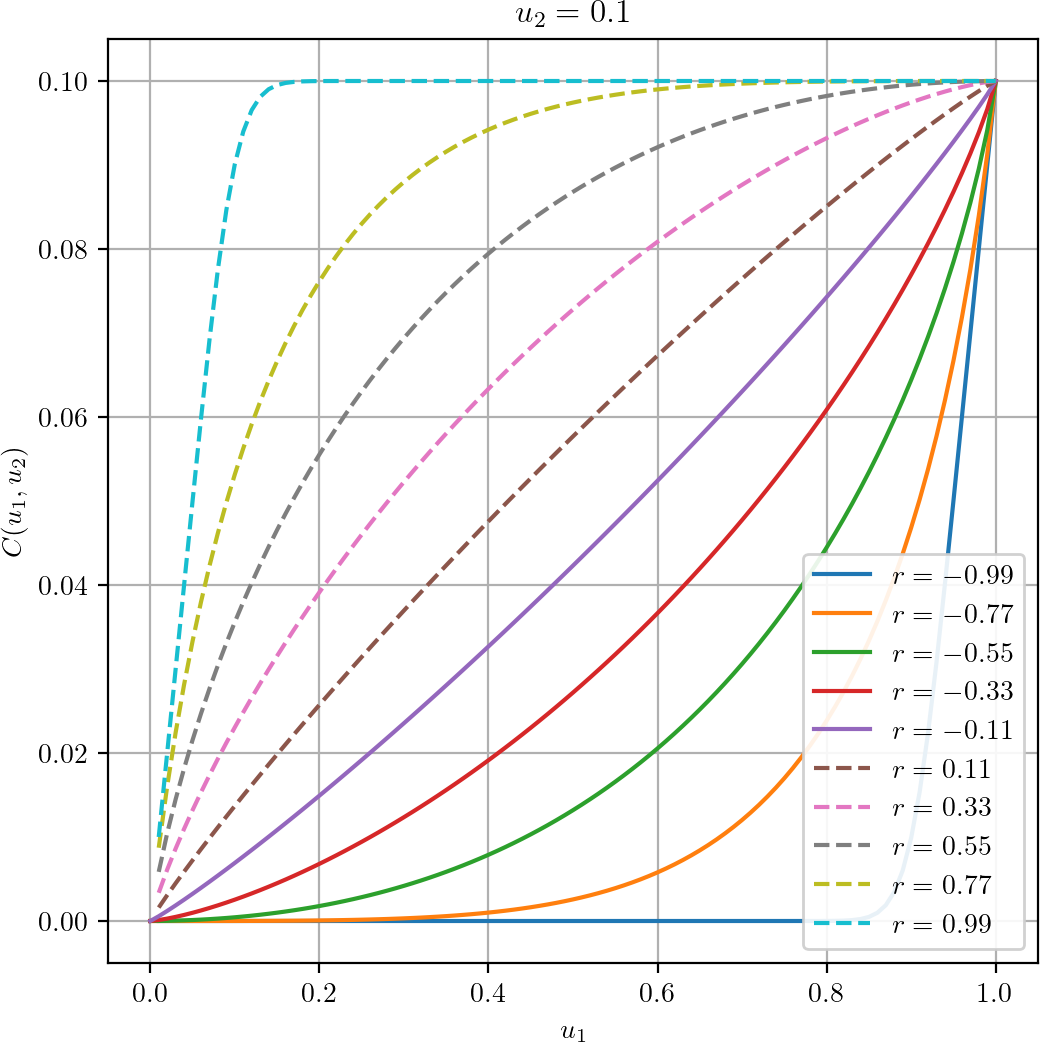
\includegraphics[width=\linewidth]{Images/Guassian_copula/gaussian_copula_0.png}
    \end{subfigure}\hfill
    \begin{subfigure}{0.4\linewidth}
        \centering
        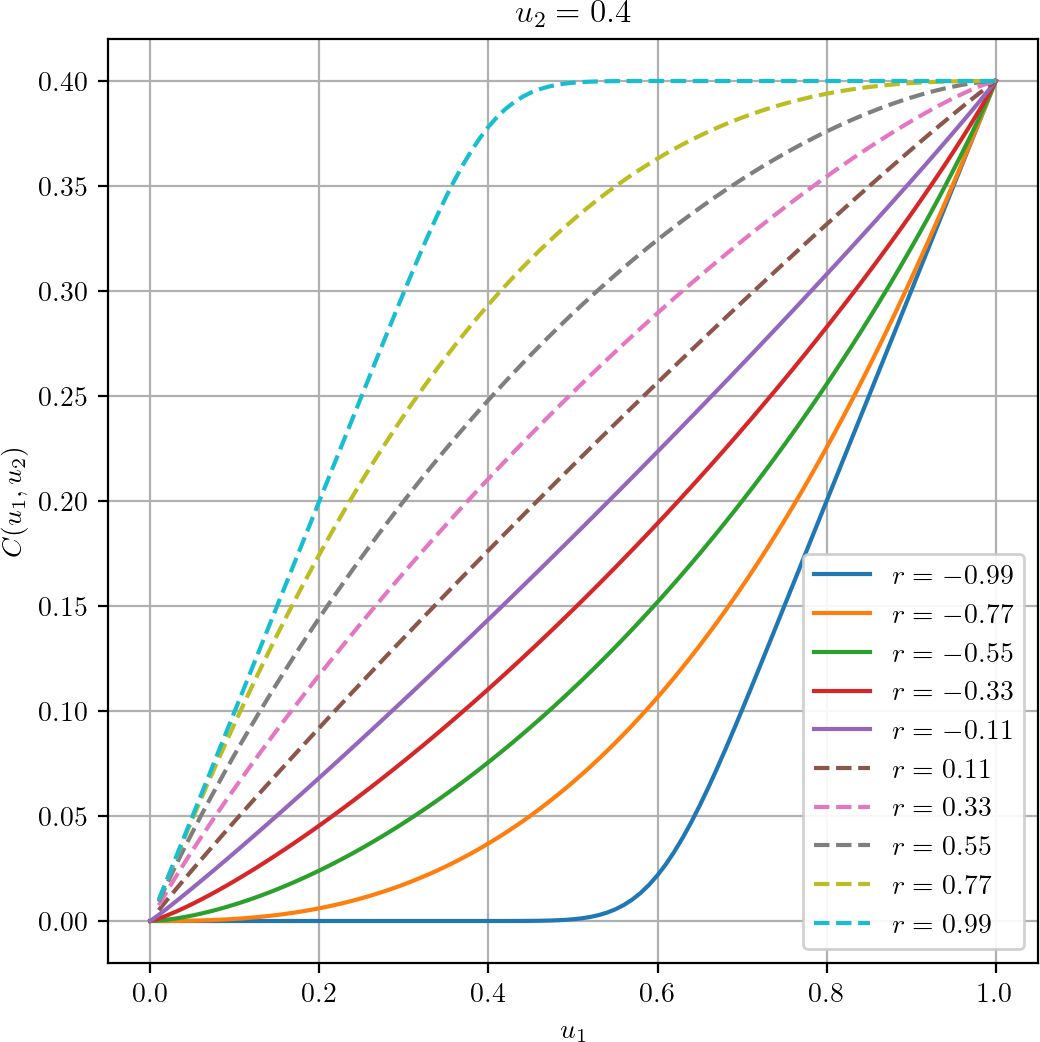
\includegraphics[width=\linewidth]{Images/Guassian_copula/gaussian_copula_1.png}
    \end{subfigure}\hfill
    \begin{subfigure}{0.4\linewidth}
        \centering
        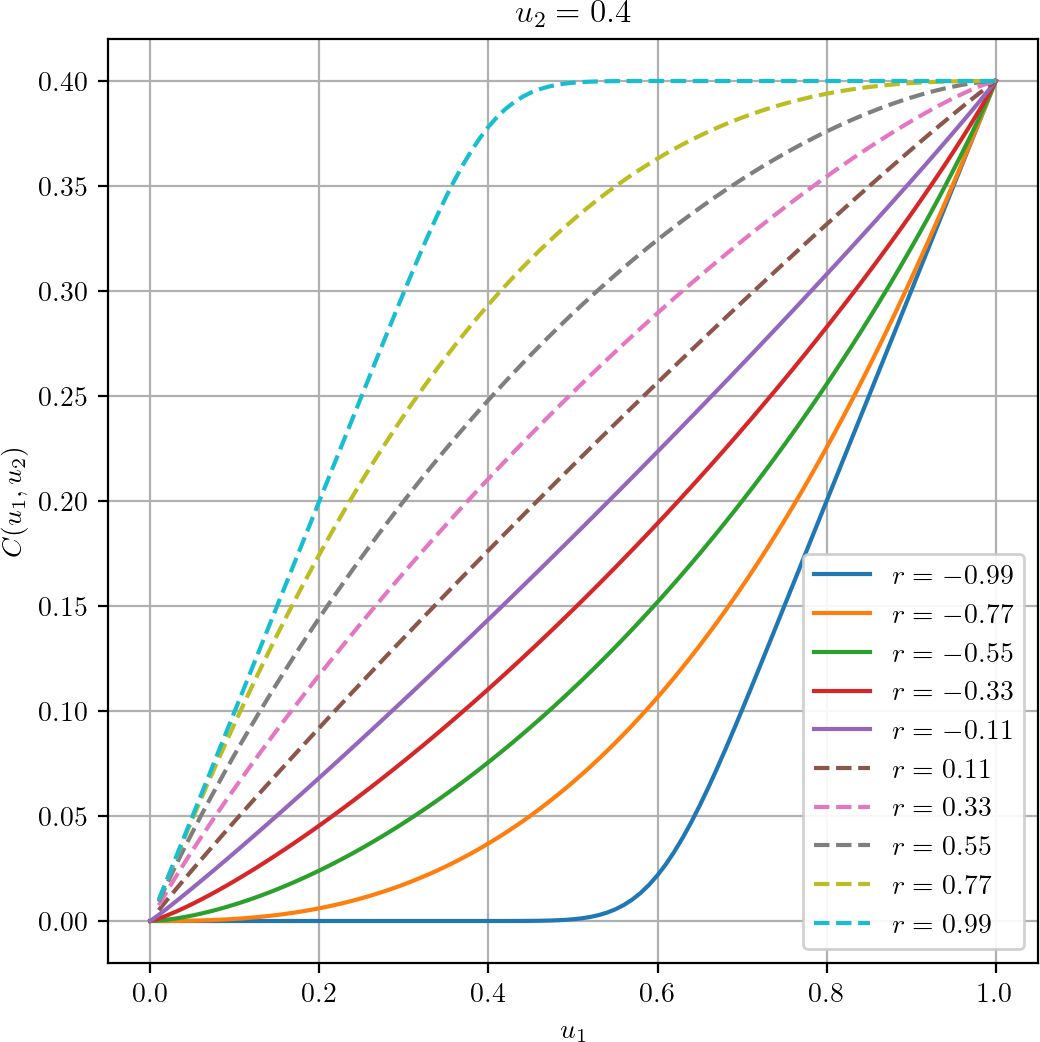
\includegraphics[width=\linewidth]{Images/Guassian_copula/gaussian_copula_2.png}
    \end{subfigure}
    \caption{Gaussian 2-copulas in the direction $u_1$ for different $u_2$. Each figure present different plots for correlations $r$ between $u_1$ and $u_2$ ranging in $[-1,1]$. Solid lines represent negative correlation, while dashed lines represent positive correlations.}
    \label{fig:gaussian_copula_simu}
\end{figure}

\begin{figure}
    \centering
    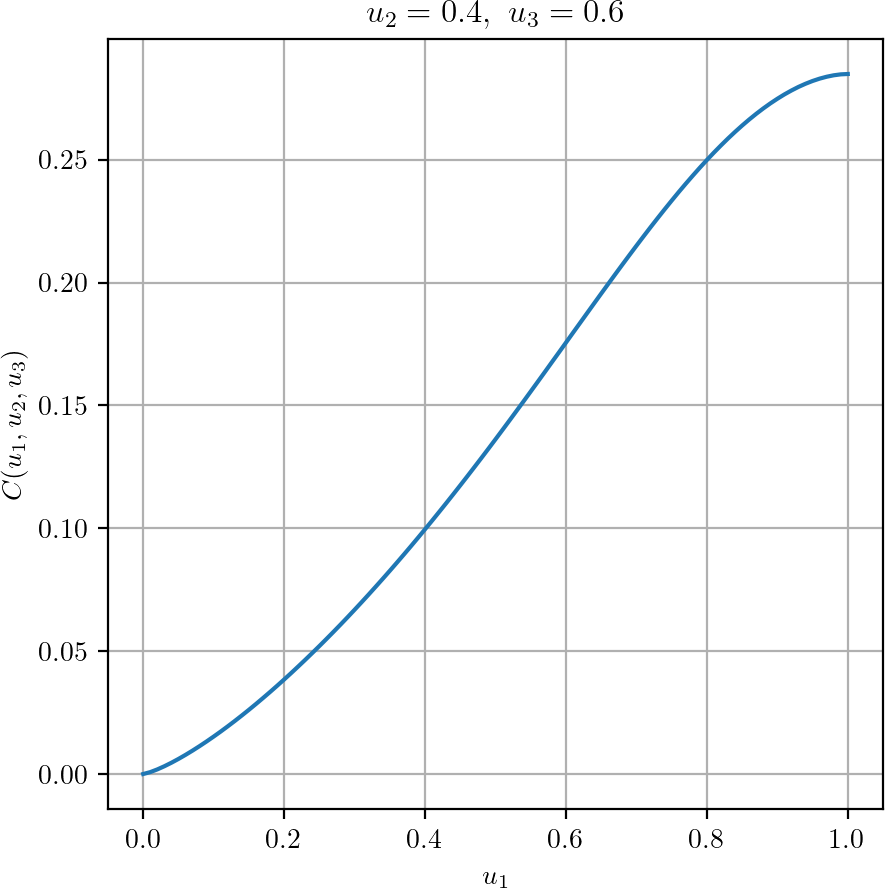
\includegraphics[width=0.5\linewidth]{Images/Guassian_copula/gaussian_copula_n3.png}
    \caption{Directional cut of a Gaussian 3-copula with in the direction $u_1$, with $R=\begin{bmatrix} 1 & -0.4 & 0.7\\ -0.4 & 1 & 0.3\\ 0.7 & 0.3 & 1 \end{bmatrix}$, $u_2=0.4$ and $u_3=0.6$. The copula is neither D-convex nor D-concave}
    \label{fig:gaussian_copula_simu_n3}
\end{figure}

The rest of this section will present some remarks and useful properties for D-convex and D-concave copulas.

\begin{remark}
    All D-convex copulas $C$ are dominated by the product copula. 
    Similarly, all D-concave copulas dominate the product copula.
\end{remark}
\begin{proof}
    Let $C$ be a D-convex copula and let $(u_1, \dots, u_n)\in[0,1]^n$.
    \begin{eqnarray*}
        C(u_1,\dots, u_n) &=& C((1-u_1)\cdot0+u_1\cdot 1, u_2, \dots, u_n)\\
        &\leqslant& (1-u_1)C(0, u_2,\dots, u_n)+u_1C(1, u_2, \dots, u_n)\\
        &=& u_1C(1, u_2,\dots, u_n)
    \end{eqnarray*}
    Doing the same for $u_2,\dots,u_n$ yields:
    \begin{eqnarray*}
        C(u_1,\dots, u_n) &\leqslant& u_1\dots u_nC(1,\dots,1) = u_1\dots u_n = C_\Pi(u_1,\dots,u_n)
    \end{eqnarray*}
    The proof for D-convexity is similar.
\end{proof}

\begin{proposition}\label{prop:sup_additivity}
    If $C$ is a D-convex copula, then it verifies for all $(u_1,\dots,u_n)\in[0,1]^n$, $(v_1,\dots,v_n)\in[0,1]^n$ \st $\forall i\in\opi1,n\cli$, $u_i+v_i\leqslant 1$:
    \begin{eqnarray}
        C(u_1,\dots,u_i+v_i,\dots,u_n)\geqslant& &C(u_1,\dots,u_i,\dots,u_n)\nonumber\\
        &+ &C(u_1,\dots,v_i,\dots,u_n)\label{eq:convex_sum}
    \end{eqnarray}
    Similarly, if $\forall i\in\opi1,n\cli$, $u_i-v_i\geqslant 0$, it verifies:
    \begin{eqnarray}
        C(u_1,\dots,u_i-v_i,\dots,u_n)\leqslant& &C(u_1,\dots,u_i,\dots,u_n)\nonumber\\
        &- &C(u_1,\dots,v_i,\dots,u_n)\label{eq:convex_diff}
    \end{eqnarray}
    The inequalities are reversed for D-concave copulas.
\end{proposition}

\begin{proof}
    Let $(u_1,\dots,u_n)\in[0,1]^n$, $(v_1,\dots,v_n)\in[0,1]^n$ \st $\forall i\in\opi1,n\cli$, $u_i+v_i\leqslant 1$. Let $i\in\opi1,n\cli$. Applying the definition of convexity \eqref{eq:convex_copula} with $v_i=0$ yields:
    \begin{eqnarray*}
        \forall t\in[0,1],~C(u_1,\dots,tu_i,\dots, u_n) \leqslant tC(u_1,\dots, u_n)
    \end{eqnarray*}
    
    Let $w_i=u_i+v_i\in ]0,1]$ (the case where $u_i=0$ or $v_i=0$ is trivial). It is possible to write $u_i=tw_i$ and $v_i=(1-t)w_i$, with $t=\frac{u_i}{w_i}\in[0,1]$. Then it holds that:
    \begin{eqnarray*}
            C(u_1,\dots,u_i,\dots,u_n) =& C(u_1, \dots, tw_i,\dots, u_n) &\leqslant tC(u_1, \dots, w_i, \dots, u_n)\\
            C(u_1,\dots,v_i,\dots,u_n) =& C(u_1, \dots, (1-t)w_i,\dots, u_n) &\leqslant (1-t)C(u_1, \dots, w_i, \dots, u_n)
    \end{eqnarray*}
    Summing the above equations yields:
    \begin{eqnarray*}
        C(u_1,\dots,u_i,\dots,u_n) + C(u_1,\dots,v_i,\dots,u_n) &\leqslant& C(u_1, \dots, w_i, \dots, u_n)\\
        &\leqslant& C(u_1, \dots, u_i+v_i, \dots, u_n)
    \end{eqnarray*}
    which proves equation \eqref{eq:convex_sum}.

    Let $w_i=u_i-v_i\in [0,1]$, clearly $w_i+v_i\leqslant1$. Using equation \eqref{eq:convex_sum}, it holds that:
    \begin{align*}
        &C(u_1,\dots,w_i,\dots,u_n) + C(u_1,\dots,v_i,\dots,u_n) &\leqslant~&C(u_1, \dots, w_i+v_i, \dots, u_n)\\
        \Leftrightarrow~ &C(u_1,\dots,w_i,\dots,u_n) &\leqslant~&C(u_1, \dots, w_i+v_i, \dots, u_n)\\
        &&&-C(u_1,\dots,v_i,\dots,u_n)\\
        \Leftrightarrow~ &C(u_1,\dots,u_i-v_i,\dots,u_n) &\leqslant~&C(u_1, \dots, u_i, \dots, u_n)\\
        &&&-C(u_1,\dots,v_i,\dots,u_n)
    \end{align*}
    which proves equation \eqref{eq:convex_diff}.
\end{proof} 

\begin{proposition}
    If $C$ is a D-convex copula, then it verifies for all $(u_1,\dots,u_n)\in[0,1]^n$, $(v_1,\dots,v_n)\in[0,1]^n$ \st $\forall i\in\opi1,n\cli$, $u_i-v_i\geqslant 0$:
    \begin{eqnarray}
        C(u_1-v_1,\dots,u_i-v_i,\dots,u_n-v_n)\leqslant& &H^{u_1,\dots,u_i,\dots,u_n}_{v_1,\dots,v_i,\dots,v_n}\label{eq:convex_diff_hvol}
    \end{eqnarray}
    where $H$ is the H-volume of $C$. The inequality is reversed for D-concave copulas.
\end{proposition}

\begin{proof}
    The result is straightforward by induction using equation \eqref{eq:convex_diff}.
\end{proof}

\section{Sampling from a Copula}
As a copula represent the CDF of a multivariate random variable, it is possible to sample from it. This section details a method for sampling from copulas in general, and a special method for sampling from copulas in the family of Gaussian copulas. Given a copula $C$, and two CDF $F_X$ and $F_Y$, a method to generate a pair of observations $(x, y)$ from a joint CDF $C(F_X, F_Y)$ is the following:

\begin{itemize}
    \item Sample two independent samples $u_1, u_2$ from a uniform distribution on [0,1]
    \item Set $v=\partial C^{-1}(u_2)$ where $\partial C^{-1}$ is the quasi-inverse of the partial derivative of $C$ regarding its first variable (which exists almost everywhere and is invertible).
    \item $(u_1, v)$ each follow a uniform distribution on $[0,1]$, and their associated copula is $C$ 
    \item The desired pair is $(x_1,x_2) = (F^{-1}_X(u_1), F^{-1}_Y(v))$, with $F_X^{-1}$, $F_Y^{-1}$ being the quasi-inverses of the marginals CDFs.
\end{itemize}

Details of this method in the $n$-dimensional case can be found in \cite{cherubini_copula_2004}. However, drawing samples from a Gaussian $n$-copula with a correlation matrix $R$ are simpler to obtain:
\begin{itemize}
    \item Compute the Cholesky decomposition $A$ of the correlation matrix $R$
    \item Draw $n$ independent random samples $u=(u_1, \dots, u_n)'$ from $\mathcal{N}(0,1)$, where $\mathcal{N}$ is the normal distribution.
    \item Set $v=Au$
    \item Set $w_k=\Phi(v_k)$ where $\Phi$ is the univariate normal cumulated distribution function
    \item The desired draw is $(x_1,\dots, x_n)=(F^{-1}_1(w_1), \dots, F^{-1}_n(w_n))$ with $F_i^{-1}$, being the quasi-inverse of the $i$-th marginal CDF.
\end{itemize}

\section{Methods for Joining credal sets with copulas}
When working with multiple sources of uncertain information, one must take into account the dependency between the different sources in order to correctly determine the joint model. Section \ref{sec:copulas} introduced copulas, a type of dependency model that we will be using for joining the uncertainty model on images intensities. We consider here $n\in\mathbb{N}^*$ uncertain variables $(X_i)_{1\leqslant i\leqslant n}$ taking values respectively in an totally ordered finite space $\X_i$. Index $i$ will usually refer to the $i$-th random variable (or random set). We note $\M_i$ the credal set representing the uncertainty of $X_i$, and $C$ a $n$-copula. Focal sets of a belief function will be noted $a^i_k$, where $k$ refers to the $k$-th focal set if they are numbered. We also note $\bigsqcup$ the union of disjoint elements.

When working with precise probabilities, a copula $C$ joins univariate Cumulative Distribution Functions (CDF), called marginals, into a mutlivariate CDF. When working with marginals modeled by Imprecise Probabilities, joining the models with a copula on the product space $\X=\X_1\tdt\X_n$ is not as straightforward. We present here three different approaches to create a multivariate credal set using a copula and imprecise marginals. 

\subsection{Point-wise aggregation}
A first way of creating a joint credal set is to sample a precise marginal for each marginal credal sets $\M_i$ and to use Sklar's theorem with the copula $C$ to create a precise multivariate CDF. The set of all resulting CDFs is thus:
\begin{eqnarray}\label{eq:robust_ancestor}
    \mathcal{S}(C,\M_i) = \{F~|~\forall x_i \in \X_i,~ F(x_1,\dots,x_n) = C(F_1(x_1), \dots, F_n(x_n))\}
\end{eqnarray} where $F_i\in\M_i$.

This set is not strictly a credal set as it is not guaranteed to be convex \cite{schmelzer_random_2023}. We thus define the joint credal set as the convex hull $\M_{robust}$ of $\mathcal{S}$:

\begin{eqnarray}\label{eq:robust_set}
    \M_{robust}(C,\M_i) = \{&&F~|~\forall A \subseteq \X,\nonumber\\
    &&\inf_{G\in\mathcal{S}(C,\M_i)}G(A)\leqslant F(A)\leqslant\sup_{G\in\mathcal{S}(C,\M_i)}G(A)~\}
\end{eqnarray}

We refer to this joint credal set as $\M_{robust}(C,\M_i)$ as it contains every element of the marginal credal sets with copula $C$ as their dependency model. We will omit ``$(C,\M_i)$'' when there are no confusion possible to avoid using heavy notations. $\M_{robust}$ is thus the smallest credal set containing $\mathcal{S}$. It is interesting to notice that it can contain additional multivariate CDFs that do not possess the copula $C$ as the dependency model of its marginals. This credal set is not easy to compute for events that are not Cartesian products of marginal cumulated events

\subsection{Copula applied to cumulated mass functions}\label{sec:joint_mass}
In this section, we will present another way of creating a joint credal set from multiple marginal ones. Consider the same copula $C$ as before and the same marginal credal sets $\M_i$. Each credal set $\M_i$ is fully determined by a mass distribution function $m_i$, which is strictly positive over its $N_i$ focal sets $a^i_1, \dots, a^i_{N_i}$. As described in \cite{ferson_dependence_2004}, it is possible to use the cumulated mass distribution functions as marginals of the copula to create a joint mass distribution function, granted that there is a complete order defined on the focal sets. Links between copulas and belief functions have been investigated in the continuous case in \cite{schmelzer_joint_2015, schmelzer_multivariate_2019}, the special case of necessity functions in \cite{schmelzer_sklars_2015} and of p-boxes in \cite{schmelzer_random_2023}.

Let suppose, without loss of generality, that the marginal focal sets are numbered according to the order $\preceq_i$: $a^i_1\preceq_ia^i_2\preceq_i\dots\preceq_i a^i_{N_i}$. The idea behind this method is to replace the precise marginal CDFs by cumulated masses, to conserve the philosophy behind Sklar's theorem. We thus first define the joint mass $m_\times$ on the product space of focal sets. Let $a_{k_i}^i$ be the $k_i$-th focal set of $m_i$ according to the chosen order. $m_\times$ is computed as the H-volume of copula $C$ computed over the cumulated marginal masses:
\begin{eqnarray}\label{eq:joint_mass}
    m_\times(a^1_{k_1}\tdt a^n_{k_n}) = H_{\sum_{k=0}^{k_1-1}m_1(a^1_k), \dots, \sum_{k=0}^{k_n-1}m_n(a^n_k)}^{\sum_{k=0}^{k_1}m_1(a^1_k), \dots, \sum_{k=0}^{k_n}m_n(a^n_k)}
\end{eqnarray}
with the convention that $\forall i,\, a^i_0=\emptyset$, which is not strictly a focal set but allows to deal with the case $k_i=1$ as $m_i(a^i_0)=0$. For sets that are not of the form $a^1_{k_1}\tdt a^n_{k_n}$, the mass $m_\times$ is null. By this definition, $m_\times$ is a correctly defined mass distribution function.
\begin{proof}
    By definition it holds that $m_\times(\emptyset)=0$, and the properties of the H-volume impose that $m_\times\in[0,1]$.
    
    There are multiple way of proving that $\sum_{A\subseteq\X}m_\times(A)=1$. A direct proof can be done in the case $n=2$, but the notations become quite for any $n>2$. Instead let us use the interpretation of a copula as a multivariate CDF. 
    Let $\forall i\in\opi 0,\, n\cli,\, F_i$ be a CDF over $[0,\, N_i]$, with, $F_i(j)=\sum_{k=0}^j m_i(a_k^i)$. By Sklar's theorem, $F=C(F_1,\dots, F_n)$ is a multivariate CDF over $[0,\, N_1]\tdt[0,\, N_n]$. Thus it holds that $F([0,\, N_1]\tdt[0,\, N_n])=1$ and:
    \begin{eqnarray*}
        F([0, N_1]\tdt[0, N_n]) &=& F([0,\dots,0])+\\
        &&F\left(\bigsqcup_{k_1=0}^{N_1-1}\dots\bigsqcup_{k_n=0}^{N_n-1}\left(]k_1, k_1+1]\tdt]k_n, k_n+1]\right)\right)\\
        &=& 0 + \sum_{k_1=0}^{N_1-1}\dots\sum_{k_n=0}^{N_n-1} F(]k_1, k_1+1]\tdt]k_n, k_n+1])\\
        && \text{(CDF of an union of disjoint elements)}\\
        &=& \sum_{k_1=0}^{N_1-1}\dots\sum_{k_n=0}^{N_n-1} H_{F_1(k_1), \dots, F_n(k_n)}^{F_1(k_1+1), \dots, F_n(k_n+1)}\\
        &=& \sum_{k_1=1}^{N_1}\dots\sum_{k_n=1}^{N_n} H_{\sum_{k=0}^{k_1-1}m_1(a^1_k), \dots, \sum_{k=0}^{k_n}m_n(a^n_k)}^{\sum_{k=0}^{k_1}m_1(a^1_k), \dots, \sum_{k=0}^{k_n}m_n(a^n_k)}\\
        &=& \sum_{(a^1_{k_1}\tdt a^n_{k_n})\subseteq\X}m_\times(a^1_{k_1}\tdt a^n_{k_n})
    \end{eqnarray*}
Therefore it holds that:
\begin{eqnarray}
    \sum_{A\subseteq\X}m_\times(A)=\sum_{(a^1_{k_1}\tdt a^n_{k_n})\subseteq\X}m_\times(a^1_{k_1}\tdt a^n_{k_n})=1
\end{eqnarray}
which proves that $m_\times$ is a mass distribution function.
\end{proof}

Having defined a mass distribution function on the product space $\X$, we thus define the joint credal set $\M_{mass}$ as: 
\begin{eqnarray}\label{eq:credal_set_mass}
    \M_{mass} = \{P~|~\forall A\subseteq\X, P(A)\geqslant \sum_{a\subseteq A}m_\times(A)\}
\end{eqnarray}

With this way of defining the multivariate mass, the choice of arbitrary orders $\preceq_i$ can have a significant impact on the value of the multivariate mass function. The next example illustrate this statement.

\begin{example}\label{ex:joint_mass}
    Let us present an example in the case $n=2$. Let $m_1$ be a mass distribution function over the power set $2^{\X_1}$ of $\X_1$ with two focal sets $a_1,\, a_2$. Similarly, let $m_2$ be a mass distribution function over the power set $\X_2$ with two focal sets $a_1^2,~a_2^2$. Throughout this example we will assume that $a_1^2\preceq_2a_2^2$. We consider the minimum copula $C(u,v)=\min(u,v)$ and $m_1(a_1^1)=m_1(a_2^1)=m_2(a_1^2)=0.5$.
    If there is no natural order on the focal sets of $m_1$, we have to chose an arbitrary one:
    \begin{itemize}
        \item[-] If "$a_1^1\preceq_1a_2^1$" is the arbitrary order (see figure \ref{fig:joint_distrib_arb}), then
        \begin{eqnarray*}
            m_\times(a_1^1,~a_1^2) &=& C(m_1(a_1^1),~m_2(a_1^2))\\
            &=& 0.5\\
            m_\times(a_2^1,~a_1^2) &=& C(1,~m_2(a_1^2)) - C(m_1(a_1^1),~m_2(a_1^2))\\
            &=& m_2(a_1^2) - C(m_1(a_1^1),~m_2(a_1^2))\\
            &=& 0
        \end{eqnarray*}
        \item[-] If "$a_2^1\preceq_1a_1^1$" is the arbitrary order, then
        \begin{eqnarray*}
            m_\times(a_1^1,~a_1^2) &=& C(1,~m_2(a_1^2)) - C(m_1(a_2^1),~m_2(a_1^2))\\
            &=& m_2(a_1^2) - C(m_1(a_2^1),~m_2(a_1^2))\\
            &=& 0\\
            m_\times(a_2^1,~a_1^2) &=& C(m_1(a_2^1),~m_2(a_1^2))\\
            &=& 0.5
        \end{eqnarray*}
    \end{itemize}
    This illustrates that different orders lead to different masses and thus to different credal sets.
    \begin{figure}[!ht]
        \centering
        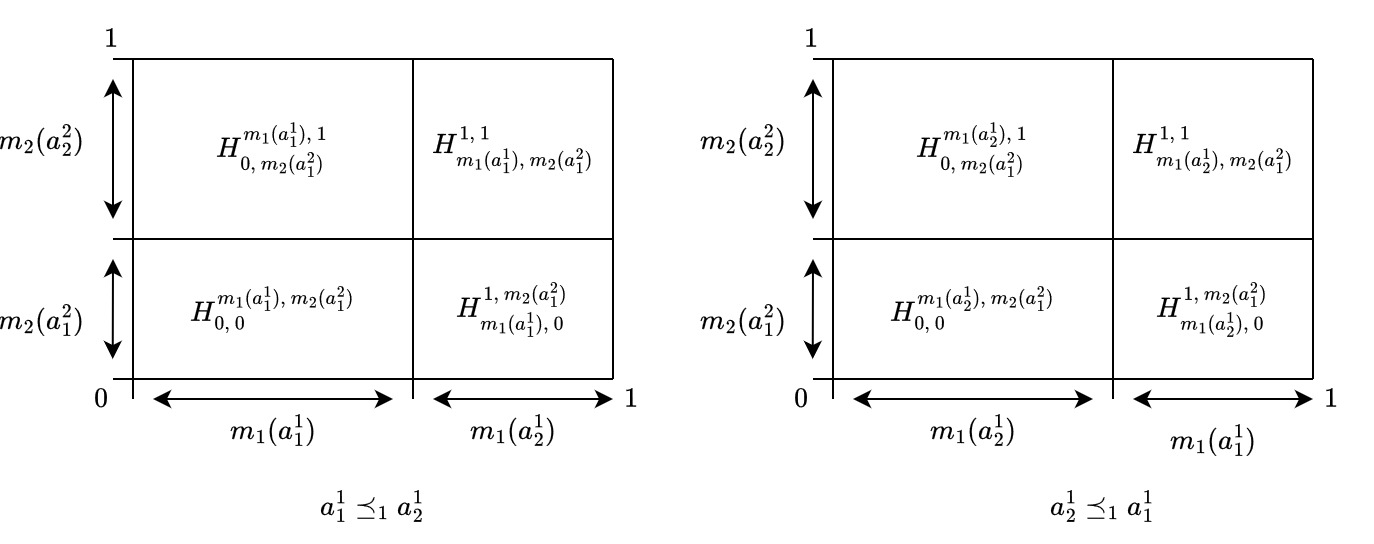
\includegraphics[width=\linewidth]{Images/M_mass_h_volume.jpg}
        \caption{H-volume diagram in the case $a_1^1\preceq_1a_2^1$}
        \label{fig:joint_distrib_arb}
    \end{figure}
\end{example}

In general, no order exists on the focal sets of belief functions, therefore an order has to be chosen arbitrarily. However, special cases of belief functions exhibit a natural order on their focal sets, for instance p-boxes and possibilities:
\begin{itemize}
    \item Focal sets of p-box are of the shape $a_\alpha = [\overline{F}^{-1}(\alpha),~\underline{F}^{-1}(\alpha)]$ (\cite{destercke_unifying_2008}), with $\alpha\in [0,1]$ and $F^{-1}$ being the inverse of a CDF (or quasi-inverse if the inverse does not exists). Thus the natural order for a p-box is $a_\alpha\preceq a_\beta \Leftrightarrow \alpha\leqslant\beta$
    \item Focal sets of possibility distributions form a nested family of sets. The natural order between the focal sets is therefore $a_1\preceq a_2 \Leftrightarrow a_1 \subseteq a_2$.
\end{itemize}

The credal set $\M_{mass}$ is different from $\M_{robust}$ as its bounds do not always coincide. This is because applying the copula to the cumulated masses instead of the CDFs encodes the correlation between sets and not between the underlying values of those sets, as it is usually done in the precise case. For instance, consider the setting of example \ref{ex:joint_mass} with $a_2^1\preceq_1a_1^1$, and suppose that the values covered by $a^1_1$ are high values in $\X_1$, and conversely that the values covered by $a^2_1$ are low values in $\X_2$. Applying the minimum copula to the cumulated masses would assign a null joint mass to $a_1^1\times a_1^2$. In the precise setting, joining two random variables in $\mathbb{R}$ with the minimum copula means that low values of the variables are positively correlated.

\subsection{Copulas applied to belief functions}
Another way of joining credal sets with a copula is by directly applying the copula to their lower envelope $\low_i$ for every event:
\begin{eqnarray}\label{eq:copula_on_lower_proba}
    \M_{agg} = \{P~|~\forall A_i\subseteq\X_i, P(A_1,\dots, A_n)\geqslant C(\low_1(A_1), \dots, \low_n(A_n)\}
\end{eqnarray}

The constraints on this set only occur on the product space $\X_1\tdt \X_n$, contrary to $\M_{mass}$. We note $\M_{agg}$ this credal set as it uses the copula as an aggregation operator only, without conserving the meaning associated to copulas by Sklar's theorem. In this regard, $\M_{agg}$ has less meaning than $\M_{robust}$ or $\M_{mass}$, but presents the advantage of being easier to compute than those joint credal sets. Figure \ref{fig:meaning_computation} sums up the performances of the different methods in terms of computation cost and meaningfulness.

\begin{figure}[!hb]
    \centering
    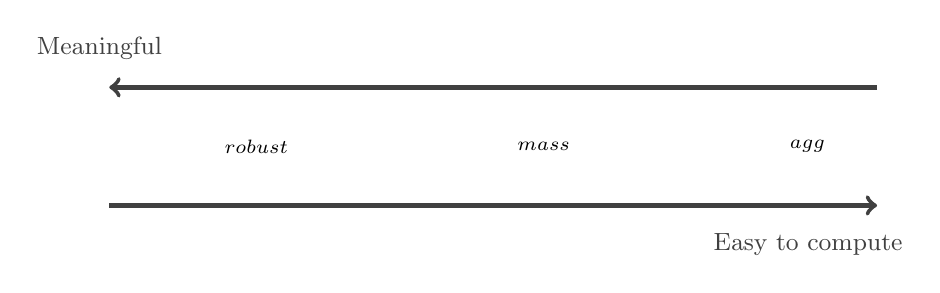
\begin{tikzpicture}[scale=1]
        \draw (0, 0) node (a) {};
        \draw (10, 0) node (b) {};
        \draw (0, 1.5) node (c) {};
        \draw (10, 1.5) node (d) {};
        
        \draw[->, ultra thick, darkgray] (a) to node[midway, left, inner sep=0.5cm] {} (b);
        \draw[->, ultra thick, darkgray] (d) to node[midway, left, inner sep=0.5cm] {} (c);
        
        \draw [darkgray] (9, -0.5) node (z) {\small Easy to compute};
        \draw [darkgray] (0, 2) node (z) {\small Meaningful};
        
        \draw (9, 0.75) node (z) {$\M_{agg}$};
        \draw (5.65, 0.75) node (z) {$\M_{mass}$};
        \draw (2, 0.75) node (z) {$\M_{robust}$};
    \end{tikzpicture}
    \caption{Comparing different methods of joining credal sets with a copula.}
    \label{fig:meaning_computation}
\end{figure}

In general, applying the copula directly to the lower probabilities as in \eqref{eq:copula_on_lower_proba} does not produce a coherent lower probability that avoid sure loss. For instance, let us consider $\X_1 = \X_2 = \{1, 2\}$, two lower previsions $\low_1$ and $\low_2$ such that $\low_1(\{1\}) = \low_1(\{2\}) = \low_2(\{1\}) = \low_2(\{2\}) = 0.5$. Joining those two lower probabilities using the minimum copula $C(u,v)=\min(u,v)$ gives a mapping $\low$ which is neither coherent nor avoid sure loss (Table \ref{tab:non_coherent_lower}).

\begin{table}[!ht]
    \centering
    \begin{tabular}{|c||c|c|}
        \hline
        \hspace{0.2cm} $\low$ \hspace{0.2cm} & \hspace{0.2cm} $\{1\}$ \hspace{0.2cm} & \hspace{0.2cm} $\{2\}$ \hspace{0.2cm} \\\hline\hline
        $\{1\}$ & $0.5$ & $0.5$ \\\hline
        $\{2\}$ & $0.5$ & $0.5$\\
        \hline
        \end{tabular}
        \caption{$\low = \min(\low_1, \low_2)$}
        \label{tab:non_coherent_lower}
\end{table}

In the special case of the product copula $C_\Pi$, the joint lower probability $\low_{C_\Pi}$ induced by \eqref{eq:copula_on_lower_proba} avoids sure loss if its marginals also avoid sure loss. It follows that for all copulas $C$ dominated by the product copula (\ie $C_\Pi\geqslant C$), and for every $\M_i$ avoiding sure loss, $\M_{agg}(C, \M_i)$ is a non empty credal set.
\begin{proof}
    For $i\in\{1,\dots,n\}$, let $\low_i$ be a lower probability avoiding sure lost, \ie whose credal set $\M_i$ contains at least one probability distribution $P_i$. Let us define a multivariate probability $P$ on every $(A_1\tdt A_n)\subseteq\X$ as:
    \begin{eqnarray*}
        P(A_1\tdt A_n) = P_1(A_1)\tdt P_n(A_n)
    \end{eqnarray*}
    Defining $P$ on $(A_1\tdt A_n)\subseteq\X$ is sufficient as those sets contain every atom of $\X$.
    Because $\forall i, P_i\in\M_i,~P_i\geqslant \low_i$, then:
    \begin{eqnarray*}
        P(A_1\tdt A_n) \geqslant \low_1(A_1)\tdt \low_n(A_n) &=& C_\Pi(\low_1(A_1), \dots, \low_n(A_n))\\
        &=& \low_{C_\Pi}(A_1\tdt A_n)
    \end{eqnarray*}
which means $P\in\M_{agg}(C_\Pi, \M_i)$. Therefore $\M_{agg}(C_\Pi, \M_i)$ avoids sure loss if every $\M_i$ avoids sure loss.

Let $C$ be a copula dominated by $C_\Pi$ (\ie $C_\Pi\geqslant C$), and $\low_C$ the lower probability associated with $\M_{agg}(C, \M_i)$. Then it holds that for all $(A_1\tdt A_n)\subseteq\X$:
\begin{eqnarray*}
\low_{C_\Pi}(A_1\tdt A_n)&=&C_\Pi(\low_1(A_1), \dots, \low_n(A_n)) \\
    &\geqslant& C(\low_1(A_1),\dots, \low_n(A_n)) = \low_C(A_1\tdt A_n)
\end{eqnarray*}
which implies that $\M_{agg}(C_\Pi, \M_i)\subseteq \M_{agg}(C, \M_i)$.
\end{proof}

Conversely, no lower probability $\low_C$ obtained using \eqref{eq:copula_on_lower_proba} with a copula $C$ strictly superior to the product copula by is guaranteed to avoid sure loss, it depends on the marginal credal sets $\low_i$.

\begin{proof}
    Let $C$ be a copula strictly superior to the product. Then there exists $(u_1,\dots,u_n)\in[0,1]^2$ such that:
    \begin{eqnarray*}
        C(u_1,\dots, u_n)~>~u_1\dots u_n
    \end{eqnarray*}
    Let $\M_i$ be marginals credal sets such that $\low_i$ are \textit{precise} probabilities, and that:
    \begin{eqnarray*}
        \forall i,~\exists A_i\in\X_i,~\low_i(A_i)=u_i
    \end{eqnarray*}
    Suppose that $\M_{agg}(C, \M_i)$ avoids sure loss, \ie there is a probability $P$ such that $P\geqslant\low_C$. Let $S$ be a collection of disjoint cylindrical sets of $\X$ covering the complementary event $(A_1\tdt A_n)^C$ of $(A_1\tdt A_n)$. $S$ is defined so that $(A_1\tdt A_n)^C=\bigsqcup_{s\in S}s$.
    Then,
    \begin{eqnarray*}
        P(\X) &=& P\left(\left(A_1\tdt A_n\right)\bigsqcup\left(A_1\tdt A_n\right)^C\right)\\
        &=& P\left(A_1\tdt A_n\right)+P\left((A_1\tdt A_n)^C\right)\\
        &=& P\left(A_1\tdt A_n\right)+\sum_{(s_1\tdt s_n)\in S}P(s_1\tdt s_n)\\
        &\geqslant& \low_C\left(A_1\tdt A_n\right)+\sum_{(s_1\tdt s_n)\in S}\low_C(s_1\tdt s_n)\\
        &>& \low_{C_\Pi}\left(A_1\tdt A_n\right)+\sum_{(s_1\tdt s_n)\in S}\low_{C_\Pi}(s_1\tdt s_n)
    \end{eqnarray*}
    Because we chose $\low_i$ so that they are precise probabilities, their product is also a precise probability. Using the fact that summing probabilities of disjoint events is equal to the probability of their union:
    \begin{eqnarray*}
        \low_{C_\Pi}\left(A_1\tdt A_n\right)+\sum_{(s_1\tdt s_n)\in S}\low_{C_\Pi}(s_1\tdt s_n) &=& \low_{C_\Pi}\left(A_1\tdt A_n\right)+\\
        &&\low_{C_\Pi}\left((A_1\tdt A_n)^C\right)\\
        &=& 1
    \end{eqnarray*}
    This means that $P(\X)>1$ which is impossible. Thus $\M_{agg}(C, \M_i)=\emptyset$ and $\M_{agg}(C, \M_i)$ does not avoid sure loss.
\end{proof}

\section{Inclusions between joint credal sets}
\comroman{small results from IJAR}
\subsection{Product copula}\label{subsection:product_copula}
In this section, we will consider the case of the product copula $C_\Pi$, representing independence between variables. Using this copula in the robust approach defined by equation \eqref{eq:robust_set} is referred as the strong product in \cite{kacprzyk_factorisation_2010}. Let us denote $\low_{robust}$ the infimum of $\M_{robust}(C_\Pi, \M_i)$ and $\mathcal{S}$ the set from which $\M_{robust}$ is computed (eq. \eqref{eq:robust_ancestor}).
For cylindrical sets $(A_1, \dots, A_n)$ of $\X$, it holds that:
\begin{eqnarray*}
    \low_{robust}(A_1\tdt A_n) &=& \inf\{P(A_1\tdt A_n)~|~P\in\mathcal{S}\}\\
    &=&\inf\{\low_1(A_1)\dots\low_n(A_n)~|~P_i\in\M_i\}\\
    &=&\inf\{\low_1(A_1)~|~P_1\in\M_1\}\dots\inf\{\low_n(A_n)~|~P_n\in\M_n\}\\
    &=&\low_1(A_1)\dots\low_n(A_n)
\end{eqnarray*}
We can split the infimum of a product as a product of infima because we consider mappings with positive values. As this is equivalent of applying the copula directly to the marginals, $\M_{robust}$ and $\M_{agg}$ have the same bounds on cylindrical events. On other events, the lower probabilities are defined as the infimum of the credal sets, thus all bounds are the same and it holds that:
\begin{eqnarray}
    \M_{robust}(C_\Pi, \M_i)=\M_{agg}(C_\Pi, \M_i)
\end{eqnarray}
\comroman{Sébastien est-ce que tu peux me confirmer cela? Jusqu'à présent on disait que $\M_{robust}\subseteq\M_{agg}$ mais je n'arrive pas à voir pourquoi l'égalité ne tiendrait pas. Il me semble que Bernhard disait dans \cite[Example 5]{schmelzer_random_2023} que ce n'était pas le cas mais je ne suis pas certain qu'on parle bien des mêmes credal sets pour commencer.}

\comseb{Non, on ne peut pas dire ça. Enfin, on peut le dire étant donné ta déf de $\M_{robust}$, mais cette dernière ne revient pas à prendre le CH d'une application point à point de la copule: elle revient à prendre la CH une fois qu'on a projeté l'application point à point sur le sous-domaine des événements. Voir le Chat pour plus d'infos ;). Mais il faut effectivement revoir la déf de $\M_{robust}$.}

\comroman{Je vois. Donc il faudrait définir $\M_{robust}$ uniquement comme dans l'équation \eqref{eq:robust_ancestor}, et laisser tomber la contrainte de convexité si j'ai bien compris. Je t'en reparlerai lundi}

In the case of the product copula $C_\Pi$, the arbitrary orders on the marginal focal sets have no impact on the value of the joint mass $m_\times$ defined in \eqref{eq:joint_mass}. If $a^1_{k_1},\dots,a^n_{k_n}$ is a focal set of $m_1,\dots,m_n$, then $m_\times$ is given by:
\begin{eqnarray}\label{eq:joint_mass_product}
    m_\times(a^1_{k_1}\tdt a^n_{k_n}) = m_1(a^1_{k_1})\dots m_n(a^n_{k_n})
\end{eqnarray}

\begin{proof}
    Equation \eqref{eq:joint_mass_product} shows that the order on marginal focal sets does not matter in the case of the product copula. We thus show that equation \eqref{eq:joint_mass_product} holds.
    For simplicity and coherence with the notations of equation \eqref{eq:hvolume}, we will note for all $i\in[0,n]$, $u^i=\sum_{k=0}^{k_i-1}m_i(a_k^i)$, $v^i_k=\sum_{k=0}^{k_i}m_i(a_k^i)$. $\Pi_{i=1}^n\{u_i, v_i\}$ will refer to the Cartesian product $\{u_1, v_1\}\times\{u_2, v_2\}\tdt\{u_n, v_n\}$ and we will note $C_\Pi$ and $H$ as the product copula and its H-volume regardless of their number of marginals. Those notations established, it holds that:
    \begin{eqnarray*}
        m_\times(a^1_{k_1}\tdt a^{n}_{k_{n}}) &=& H_{u_1, \dots, u_{n}}^{v_1, \dots, v_{n}}\\
        &=&\sum_{\substack{(w_1, \dots, w_{n})\in\\\Pi_{i=1}^{n}\{u_i, v_i\}}}(-1)^{|\{k~|~w_k=u_k\}|}C_\Pi(w_1, \dots, w_{n})\\
        &=&\sum_{\substack{(w_1, \dots, w_{n-1})\in\\\Pi_{i=1}^{n-1}\{u_i, v_i\}}}(-1)^{|\{k~|~w_k=\sum_{k=0}^{k_i-1}m_i(a^i_k)\}|}(w_1 \dots w_{n-1}v_{n})\\
        && + \sum_{\substack{(w_1, \dots, w_{n-1})\in\\\Pi_{i=1}^{n-1}\{u_i, v_i\}}}(-1)^{|\{k~|~w_k=\sum_{k=0}^{k_i-1}m_i(a^i_k)\}|+1}(w_1 \dots w_{n-1}u_n)\\
        &=& v_{n}H_{u_1, \dots, u_{n-1}}^{v_1, \dots, v_{n-1}} - u_{n}H_{u_1, \dots, u_{n-1}}^{v_1, \dots, v_{n-1}}\\
        &=& m_{n}(a^{n}_{k_{n}})H_{u_1, \dots, u_{n-1}}^{v_1, \dots, v_{n-1}}
    \end{eqnarray*}
    Doing the same procedure for every variable leads to:
    \begin{eqnarray*}
        m_\times(a^1_{k_1}\tdt a^n_{k_n}) = m_1(a^1_{k_1})\dots m_n(a^n_{k_n})
    \end{eqnarray*}
    which concludes the proof.
\end{proof}

The mass $m_\times$ corresponds to the notion of random set independence presented in \cite{couso_survey_2000}. Let $\mathrm{Bel}_\times$ be the belief function associated to $m_\times$, and $\forall i\in[1,n], \mathrm{Bel}_i$ the mass function associated to $m_i$. Then for cylindrical sets $(A_1, \dots, A_n)$ of $\X$, it holds that:
\begin{eqnarray}
    \mathrm{Bel}_\times(A_1\tdt A_n) &=& \sum_{(a^1\tdt a^n)\subseteq (A_1, \dots, A_n)}m_\times(a^1\tdt a^n)\nonumber\\
    &=& \sum_{(a^1\tdt a^n)\subseteq (A_1, \dots, A_n)}m_1(a_1)\dots m_n(a^n)\nonumber\\
    &=& (\sum_{a^1\subseteq A_1}m_1(a^1))\dots(\sum_{a^n\subseteq A_n}m_n(a^n))\nonumber\\
    &=& \mathrm{Bel}_1(A_1)\dots \mathrm{Bel}_n(A_n)
\end{eqnarray}

This means that in the case of the product copula $C_\Pi$ with marginals being belief functions, $\M_{robust},~\M_{mass}$ and $\M_{agg}$ all coincide on cylindrical sets. Thus,
\begin{eqnarray*}
    \M_{mass}\subseteq\M_{agg}
\end{eqnarray*}

\subsection{Natural ordering of necessity functions}\label{subsec:necessity_functions}
Necessity functions $\mathrm{Nec}$, also called minitive belief functions, are a special type of belief function verify $\mathrm{Nec}(A\cap B) =\min(\mathrm{Nec}(A), \mathrm{Nec}(B))$ for all events $A, B$ in their domain of definition. In the multivariate case, when a belief is only defined on cylindrical sets, then the minitive property becomes:
\begin{eqnarray}
    &&\forall (A_1\tdt A_n)\subseteq\X, (B_1\tdt B_n)\subseteq\X,\nonumber\\
    &&\mathrm{Nec}(A_1\cap B_1,\dots, A_n\cap B_n) = \min_{(S_1,\dots,S_n)\in\Pi_i\{A_i,B_i\}}(\mathrm{Nec}(S_1, \dots, S_n))
\end{eqnarray}
In \cite{schmelzer_joint_2015}, the author showed that in order to describe the relation between a multivariate belief function and its marginals, in the bivariate case, it is necessary to use a family of sub-copulas (one copula for each tuple of increasing family of events).

\begin{theorem}[Sklar's theorem for belief functions \cite{schmelzer_joint_2015}]\label{theorem:sklar_belief}
    Let $\mathrm{Bel}:2^{\X_1}\times2^{\X_2}\rightarrow[0,1]$ be a bivariate belief function and let $\mathrm{Bel}_1$ and $\mathrm{Bel}_2$ denote its marginals over $2^{\X_1}$ and $2^{\X_2}$ respectively. Furthermore, let $\mathcal{I}_1$ and $\mathcal{I}_2$ denote increasing families of subsets of $\X_1$ and $\X_2$. Then there exists a unique subcopula $C^{\mathcal{I}_1,\mathcal{I}_2}$ on  $\mathrm{Bel}_1(\mathcal{I}_1)\times \mathrm{Bel}_2(\mathcal{I}_2)$ such that:
    \begin{eqnarray}
        \mathrm{Bel}(L_1, L_2) = C^{\mathcal{I}_1,\mathcal{I}_2}(\mathrm{Bel}_1(L_1), \mathrm{Bel}_2(L_2))
    \end{eqnarray}
    for all $L_1\in\mathcal{I}_1,L_2\in\mathcal{I}_2$.
\end{theorem}
For the reverse to be true, it is necessary that $\X_1\in\mathcal{I}_1, \X_2\in\mathcal{I}_2$. Example 1 of \cite{schmelzer_joint_2015} illustrate the need of a copula for each increasing family of events.

Necessity functions are completely determined by their focal sets which form an increasing family of events. Thus by applying Sklar's theorem for belief functions (theorem \ref{theorem:sklar_belief}), it holds that joining two necessity functions with a copula $C$ as in \eqref{eq:copula_on_lower_proba} yields a bivariate belief function (which is not necessarily a necessity function):
\begin{equation}
    \mathrm{Bel} = C(\mathrm{Nec}_1, \mathrm{Nec}_2)\label{eq:sklar_on_necessity}
\end{equation}
where $\mathrm{Nec}_1$ and $\mathrm{Nec}_2$ are the marginal necessity functions. The proof of those results where shown in \cite{schmelzer_joint_2015,schmelzer_sklars_2015}. In the following, we will consider that the focal sets $a^i$ of a necessity functions $\mathrm{Nec}_i$ are already ranked using the natural ordering $\preceq_i$:
\begin{eqnarray}
    \forall (k,j)\in[1, N_i]^2,~k\leqslant j ~\Leftrightarrow ~ a^i_k \preceq_i a^i_j ~\Leftrightarrow ~ a^i_k\subseteq a^i_j
\end{eqnarray}

\begin{proposition}\label{prop:sklar_necessity}
    Given two marginal necessity functions $\mathrm{Nec}_1, \mathrm{Nec}_2$ and a copula $C$, joining them using the copula $C$ as in \eqref{eq:sklar_on_necessity} or using the bivariate mass function as in \eqref{eq:joint_mass} with the natural inclusion ordering yields the same bivariate belief function $\mathrm{Bel}$.
\end{proposition}

\begin{proof}
    If we denote by $\mathrm{Bel}_\times$ the belief function defined in \eqref{eq:joint_mass} where the ordering is the inclusion ordering $\preceq_i$ for $i\in[1,2]$. For convenience and with respects to the notations of equation \eqref{eq:hvolume}, we note: $u^i_k=\sum_{j=0}^{k}m_i(a_j^i)$ and consider that $a^i_0=\emptyset$.
    For all focal elements $a_k^1$ of $\mathrm{Nec}_1$ and $a^2_j$ of $\mathrm{Nec}_2$, it holds that:
    \begin{eqnarray*}
        \mathrm{Bel}_\times(a^1_k, a^2_j) &=& \sum_{a^1_p\subseteq a_k^1}\sum_{a^2_q\subseteq a_j^2}m_\times(a^1_p, a^2_q) = \sum_{p=1}^k\sum_{q=1}^j m_\times(a^1_p, a^2_q)\\
        &=&\sum_{p=1}^k\sum_{q=1}^j (~C(u^1_p, u^2_q) + C(u^1_{p-1}, u^2_{q-1}) \\
        &&- C(u^1_{p-1}, u^2_{q}) - C(u^1_{p}, u^2_{q-1})~)\\
        &=&\sum_{p=1}^k\sum_{q=1}^jC(u^1_p, u^2_q) + \sum_{p=0}^{k-1}\sum_{q=0}^{j-1}C(u^1_p, u^2_q) \\
        &&- \sum_{p=0}^{k-1}\sum_{q=1}^jC(u^1_p, u^2_q) - \sum_{p=1}^k\sum_{q=0}^{j-1}C(u^1_p, u^2_q)\\
        &=& C(u^1_k, u^2_j) = C\left(\mathrm{Nec}_1(a_k^1), \mathrm{Nec}_2(a_j^2)\right)\\
    \end{eqnarray*}
    This is the case for necessity function but not in general where:
    \begin{align*}
        \sum_{a^1_p\subseteq a_k^1}\sum_{a^2_q\subseteq a_j^2}m_\times(a^1_p, a^2_q) \neq \sum_{p=1}^k\sum_{q=1}^j m_\times(a^1_p, a^2_q)
    \end{align*}
\end{proof}

\begin{proposition}
    Let $m_\times$ be a joint mass obtained using \eqref{eq:joint_mass}. If $m_\times$ verifies
    \begin{align*}
        \sum_{a^1_p\subseteq a_k^1}\sum_{a^2_q\subseteq a_j^2}m_\times(a^1_p, a^2_q) = \sum_{p=1}^k\sum_{q=1}^j m_\times(a^1_p, a^2_q)
    \end{align*}
    for all marginal focal sets $a^1_k,a^2_j$ then its marginals masses correspond to necessity functions. The reverse implication is immediate if we use the natural inclusion order.
\end{proposition}
\begin{proof}
    Let $m_\times$ be a joint mass obtained using \eqref{eq:joint_mass}, with marginal focal sets $(a^1_k)_{1\leqslant k\leqslant N_1}$, $(a^2_j)_{1\leqslant j\leqslant N_2}$ and marginal masses $m_1,m_2$. 
    Let $\mathrm{Bel}_\times$ be its associated belief function verifying
    \begin{align*}
        \sum_{a^1_p\subseteq a^1_k}\sum_{a^2_q\subseteq a_j^2}m_\times(a^1_p, a^2_q) = \sum_{p=1}^k\sum_{q=1}^j m_\times(a^1_p, a^2_q)
    \end{align*}
    for all marginal focal sets $a^1_k,a^2_j$. It is easy to check that
    \begin{align*}
        \sum_{a^2_q\subseteq \X_2}m_\times(a^1_p, a^2_q)=m_1(a^1_p)=\sum_{q=1}^{N_2}m_\times(a^1_p, a^2_q)    
    \end{align*}
    (as we sum the H-volume over a complete partition of $[0,1]$). Thus it holds that:
    \begin{align*}
        \sum_{p=1}^k m_1(a^1_p) = \mathrm{Bel}_\times(a^1_k,\X_2)=\sum_{a^1_p\subseteq a_k^1}m_1(a^1_p)
    \end{align*}
    This result is not sufficient to prove the inclusion of focal sets (there could be a set $a^1_p\subseteq a^1_k,~p>k$ with the same mass value than another set $a^1_{p'}\not\subseteq a^1_k,~p' < k$). Let us show by induction that for all $(k, p)\in\opi1,N_1\cli^2$, $a_1\subset\dots\subset a_k$ and $a_p\not\subseteq a_k$ if $p>k$.
    For the case $k=1$, it holds that:
    \begin{align*}
        \sum_{p=1}^1m_1(a^1_p) &= \sum_{a_p\subseteq a_1}m_1(a^1_p)\\
        \Leftrightarrow m_1(a^1_1) &= m_1(a^1_1) + \sum_{a^1_p\subset a^1_1}m_1(a^1_p)\\
        \Leftrightarrow 0 &=\sum_{a_p\subset a_1}m_1(a^1_p)
    \end{align*}
    which means that no focal set is a strict subset of $a_1$.
    Suppose that there is $k\in\opi1,N_1\cli$ such that: $a_1\subset\dots\subset a_k$ and $\forall p>k,~a_p\not\subseteq a_k$. In particular, $a_{k+1}\not\subseteq a_k$. It holds that:
    \begin{align*}
        \sum_{p=1}^{k+1}m_1(a^1_p) &= \sum_{a^1_p\subseteq a^1_{k+1}}m_1(a^1_p)\\
        \Leftrightarrow m_1(a^1_{k+1}) + \sum_{p=1}^{k} m_1(a^1_p) &= \sum_{a^1_p\subseteq a^1_{k+1}}m_1(a^1_p)\\
        \Leftrightarrow m_1(a^1_{k+1}) + \sum_{a^1_p\subseteq a^1_k} m_1(a^1_p) &= \sum_{a^1_p\subseteq a^1_{k+1}}m_1(a^1_p)\\
        \implies m_1(a^1_{k+1}) &= \sum_{\substack{a^1_p\subseteq a^1_{k+1} \\ a^1_p\not\subseteq a^1_k}} m_1(a^1_p)\\
        \implies m_1(a^1_{k+1}) &= m_1(a^1_{k+1}) + \sum_{\substack{a^1_p\subset a^1_{k+1} \\ a^1_p\not\subseteq a^1_k}} m_1(a^1_p)\\
        \Leftrightarrow 0 &= \sum_{\substack{a^1_p\subset a^1_{k+1} \\ a^1_p\not\subseteq a^1_k}} m_1(a^1_p)
    \end{align*}
    Which means that either there is no focal set that is a strict subset of $a^1_{k+1}$, or that they are all included in $a^1_{k}$. The first case is discarded as:
    \begin{align*}
        \sum_{a^1_p\subseteq a^1_{k+1}}m_1(a^1_p) &= \sum_{p=1}^{k+1}m_1(a^1_p)\\
        \Leftrightarrow \sum_{a^1_p\subset a^1_{k+1}}m_1(a^1_p) &= \sum_{p=1}^{k}m_1(a^1_p)>0
    \end{align*}
    thus $a_1\subset\dots\subset a_{k+1}$.
    Finally, it also holds that:
    \begin{align*}
        \sum_{a^1_p\subseteq a^1_{k+1}}m_1(a^1_p) &= \sum_{p=1}^{k+1}m_1(a^1_p)\\
        \implies \sum_{\substack{a^1_p\subseteq a^1_{k+1} \\ p>k+1}} m_1(a^1_p) + \sum_{\substack{a^1_p\subseteq a^1_{k+1} \\ p\leqslant k+1}} m_1(a^1_p) &= \sum_{p=1}^{k+1}m_1(a^1_p)\\
        \Leftrightarrow \sum_{\substack{a^1_p\subseteq a^1_{k+1} \\ p>k+1}} m_1(a^1_p) &= 0\\
    \end{align*}
    meaning that for all $p>k+1$, $a^1_p\not\subseteq a^1_{k+1}$ which ends the proof by induction. Because all focal sets form a nested family of sets, $\mathrm{Bel}_1$ is a necessity function. The proof for $\mathrm{Bel}$ is identical. 
\end{proof}

Proposition \ref{prop:sklar_necessity} holds for $n$ marginals, not covered in \cite{schmelzer_sklars_2015}. For every cylindrical set $(A_1, \dots, A_n)\subseteq\X$:
\begin{eqnarray}
    \mathrm{Bel}_\times(A_1\tdt A_n) = C\left(\mathrm{Nec}_1(A_1), \dots, \mathrm{Nec}_n(A_n)\right)
\end{eqnarray}

\begin{proof}
    The proof is similar to the one of equation \eqref{eq:joint_mass}, but this time computing the mass of $(a_{k_1}^1\tdt a_{k_n}^n)$ using $F([0,k_1]\tdt[0,k_n])$ and noticing that \begin{eqnarray*}
        \sum_{(a^1_{p_1}\tdt a^n_{p_n})\subseteq(a^1_{k_1}\tdt a^n_{k_n})}m_\times(a^1_{p_1}\tdt a^n_{p_n})=\sum_{p_1=1}^{k_1}\dots\sum_{p_n=1}^{k_n} m_\times(a^1_{p_1}\tdt a^n_{p_n})
    \end{eqnarray*} because all marginals are necessity functions, and the natural inclusion ordered is used for ranking their focal sets.
\end{proof}

As the lower probabilities of $\M_{agg}$ and $\M_{mass}$ coincide on cylindrical sets, the following set equality holds for credal sets $\M_i$ whose lower probabilities are necessity functions:
\begin{eqnarray}\label{eq:inclusion_necessity}
    \M_{mass}(C, \M_i) \subseteq \M_{agg}(C, \M_i)
\end{eqnarray}

Without further assumptions, there is no inclusion relations between $\M_{robust}$ and $\M_{agg}$ or $\M_{mass}$. The following examples present cases where $\inf\M_{robust}<\inf\M_{agg}$ or $\inf\M_{mass}<\inf\M_{robust}$, proving that it is not always possible to get an (inner or outer) approximation of $\M_{robust}$ using $\M_{mass}$ or $\M_{agg}$.

\begin{example}\label{ex:necessity}
    Let $n=2$. Consider $\X_1=\{x^1_1, x^1_2\}$ and $\X_2=\{x^2_1, x^2_2\}$. Let us define two possibility distribution $\pi_1$ and $\pi_2$ over $\X_1$ and $\X_2$ respectively, such that:

    \begin{eqnarray*}
    \begin{cases}
        \pi_1(x^1_1) = 0.1\\
        \pi_1(x^1_2) = 1
    \end{cases}
    \qquad\text{ and }\qquad
    \begin{cases}
        \pi_2(x^2_1)=1\\
        \pi_2(x^2_2)=0.1
    \end{cases}
    \end{eqnarray*}
    
    For $i\in\{1,2\}$, $\pi_i$ generates a necessity measure $\mathrm{Nec}_i$, a possibility measure $\Pi_i$ and a credal set $\M_i$. Let $P_1$ and $P_2$ be two probabilities respectively included in $\M_1$ and $\M_2$,  whose values are indicated in Table \ref{tab:proba_distrib_1}. 
    
    \begin{table}[!ht]
        \centering
        \begin{tabular}{|c|c|c|}
            \hline
            $\X_1$ & $x^1_1$ & $x^1_2$\\
            \hline\hline
            $\mathrm{Nec}_1$ & 0 & 0.9\\
            \hline
            $P_1$  & 0.1 & 0.9\\
            \hline
            $\Pi_1$ & 0.1 & 1\\
            \hline
        \end{tabular}
        \quad
        \begin{tabular}{|c|c|c|}
            \hline
            $\X_2$ & $x^2_1$ & $x^2_2$\\
            \hline\hline
            $\mathrm{Nec}_2$ & 0.9 & 0\\
            \hline
            $P_2$  & 0.9 & 0.1\\
            \hline
            $\Pi_2$ & 1 & 0.1\\
            \hline
        \end{tabular}
        \caption{Probability distributions over $\X_1$ and $\X_2$}
        \label{tab:proba_distrib_1}
    \end{table}
    
    We first consider here the Minimum copula $C_M(u,v)=\min(u,v)$. After joining $P_1$ and $P_2$ with $C_M$ to obtain a joint probability $P_\times$, let us compare its value with the value of the bivariate necessity function $C_M(\mathrm{Nec}_1, \mathrm{Nec}_2)$ on the same event $\{x_2\}\times\{y_1\}$.
    \begin{eqnarray*}
        \mathrm{Bel}_\times(\{x^1_2\}\times\{x^2_1\}) &=& C_M\left(\mathrm{Nec}_1(\{x^1_2\}), \mathrm{Nec}_2(\{x^2_1\})\right)\\
        &=& \min(0.9,~0.9) = 0.9\\
        P_\times(\{x^1_2\}\times\{x^2_1\}) &=& C_M(P_1(\X_1), P_2(\{x^2_1\})) - C_M(P_1(\{x^1_1\}),P_2(x^2_1))\\
        &=& \min(1,~0.9) - \min(0.1,~0.9) = 0.8
    \end{eqnarray*}
    
    We have $P_\times\in\M_{robust}, ~P_\times\not\in\M_{mass}$, which proves that ${M}_{robust}\not\subseteq\M_{mass}$.
    
    Let us now compare the lower bound of $\underline{P}$ of $\M_{robust}$ with that of $\M_{agg}$ but considering the \L ukasiewicz copula $C_L(u,v)=\max(u+v-1,0)$:
    \begin{eqnarray*}
        \mathrm{Bel}_\times(\{x^1_2\}\times\{x^2_1\}) &=& C_L(\mathrm{Nec}_1(\{x^1_2\}), \mathrm{Nec}_2(\{x^2_1\}))\\
        &=& \max(0,~0.9 + 0.9 - 1) = 0.8\\
        \low(\{x^1_2\}\times\{x^2_1\}) &=& \inf_{P_1\in\M_1, P_2\in\M_2}\{C_L(P_1(\{\X_1\}),~P_2(\{x^2_1\})) - C_L(P_1(\{x^1_1\}),~P_2(\{x^2_1\}))\}\\
        &=& \inf_{P_1\in\M_1, P_2\in\M_2}\{\max(0,~P_1(\X_1) + P_2(\{x^2_1\}) - 1)\\
        && - \max(0,~P_1(\{x^1_1\}) + P_2(\{x^2_1\}) -1)\}\\
        &=& \inf_{P_1\in\M_1, P_2\in\M_2}\{P_2(\{x^2_1\}) - \max(0,~P_1(\{x^1_1\}) + P_2(\{x^2_1\}) - 1 )\}\\
        &=& \inf_{P_1\in\M_1, P_2\in\M_2}\max(P_2(\{x^2_1\}),~P_2(\{x^2_1\})-P_1(\{x^1_1\}) - P_2(\{x^2_1\}) + 1 )\\
        &\geqslant& \min(\inf_{P_2\in\M_2}\{P_2(\{x^2_1\})\},~\inf_{P_1\in\M_1}\{1-P_1(\{x^1_1\})\}) = 0.9
    \end{eqnarray*}
    
    On this event $\low>Nel_\times$ and because the belief function is coherent then $\M_{mass}\not\subseteq\M_{robust}$ and $\M_{agg}\not\subseteq\M_{robust}$.
\end{example}

\subsection{Natural ordering of P-boxes}\label{subsec:pboxes}
P-boxes are special cases of belief functions that resemble the most classical CDFs. They are defined with two CDF $\underline{F},~\overline{F}$ such that $\underline{F}\leqslant\overline{F}$, their focal sets $a_\alpha$ are of the form $a_\alpha=[\overline{F}^{-1}(\alpha), \underline{F}^{-1}(\alpha)]$ with $\alpha\in[0,1]$ \cite{destercke_unifying_2008}, where $F^{-1}$ is the inverse of a CDF (or pseudo-inverse if not properly defined). It it thus possible to define a natural order on the focal sets. Let $a_\alpha$ and $a_\beta$ be two focal sets of a p-box $[\underline{F},~\overline{F}]$, with $(\alpha,\beta)\in[0,1]^2$. The natural order $\preceq$ on the focal sets is defined as follows:
\begin{align}
    a_\alpha\preceq a_\beta ~\Leftrightarrow~ \overline{F}^{-1}(\alpha)\leqslant\overline{F}^{-1}(\beta) \text{ and } \underline{F}^{-1}(\alpha)\leqslant\underline{F}^{-1}(\beta)~\Leftrightarrow~ \alpha\leqslant\beta\label{eq:order_pbox}
\end{align}

As it is the case for necessity functions, it is possible to find cases where the sets $\M_{robust}\not\subseteq \M_{mass}$ or $\M_{agg}\not\subseteq\M_{mass}$.
\begin{example}\label{ex:pbox}
    Consider the following p-boxes:
    \begin{table}[!ht]
        \centering
        \begin{tabular}{|c|c|c|}
            \hline
            $\X_1$ & $x^1_1$ & $x^1_2$\\
            \hline\hline
            $\underline{F}_1$ & 0 & 1\\
            \hline
            $\overline{F}_1$ & 0.1 & 1\\
            \hline
        \end{tabular}
        \quad
        \begin{tabular}{|c|c|c|}
            \hline
            $\X_2$ & $x^2_1$ & $x^2_2$\\
            \hline\hline
            $\underline{F}_2$ & 0.9 & 1\\
            \hline
            $\overline{F}_2$ & 1 & 1\\
            \hline
        \end{tabular}
        \caption{P-boxes over $\X_1$ and $\X_2$}
        \label{tab:example_pbox}
    \end{table}
    The p-boxes from \ref{tab:example_pbox} lead to the same belief functions as in example \ref{ex:necessity}, thus leading to the same conclusions \ie ${M}_{robust}\not\subseteq\M_{mass}$, $\M_{mass}\not\subseteq\M_{robust}$ and $\M_{agg}\not\subseteq\M_{robust}$.
\end{example}

As stated previously, p-boxes are very closely related to CDF which can motivate one to apply Sklar's therorem (\ref{theorem:sklar}) to the lower CDF and upper CDF respectively. Given $n$ p-boxes $[\underline{F}_1,~\overline{F}_1],~\dots,~[\underline{F}_n,~\overline{F}_n]$ defined over $\X_1,\dots,\X_n$ and a copula $C$, we can define the lower and upper bounds of a $n$ variate CDF as:
\begin{align*}
    \underline{F}_\times&=C(\underline{F}_1,\dots, \underline{F}_n)\\
    \overline{F}_\times&=C(\overline{F}_1,\dots, \overline{F}_n)
\end{align*}
Sklar's theorem states that $\underline{F}_\times$ and $\overline{F}_\times$ are both CDF, which means that $[\underline{F}_\times, \overline{F}_\times]$ is a multivariate p-box \cite{pelessoni_bivariate_2016, montes_sklars_2015} over cylindrical sets, defining a credal set $\M$. Clearly, the bounds of $\M_{robust}$ on cumulated events are the same as those of the credal set $\M$ induced by the multivariate p-box $[C(\underline{F}_1,\dots, \underline{F}_n),~C(\overline{F}_1,\dots, \overline{F}_n)]$.

\begin{proposition}\label{prop:convexity_pbox}
    When considering the natural order on p-boxes \eqref{eq:order_pbox} when joining masses with a copula $C$, then it holds that:
    \begin{itemize}
        \item if $C$ is D-convex, then $\M_{mass}\subseteq \M_{agg}$.
        \item if $C$ is D-concave then $\M_{agg}\subseteq\M_{mass}$ 
    \end{itemize}
\end{proposition}
Figure \ref{fig:copula_convex} illustrates the difference between $\mathrm{Bel}_\times$ and $\underline{P}$ in the case $n=2$.
\begin{proof}
    Consider $n$ p-boxes $[\underline{F}_1,~\overline{F}_1],~\dots,~[\underline{F}_n,~\overline{F}_n]$, a D-convex copula $C$ and the natural order on focal sets $(a^i_k)_{1\leqslant k \leqslant N_i}$ of each marginal p-box $[\underline{F}_i,~\overline{F}_i]$. We will denote $m_\times$ the joint mass functions obtained using equations \eqref{eq:joint_mass} and $\mathrm{Bel}_\times$ its associated belief function. We will also refer to $\underline{P}$ as the lower probability associated to $\M_{agg}$ from equation \eqref{eq:copula_on_lower_proba}.

    When considering the natural order on focal sets of a p-box \eqref{eq:order_pbox}, it holds that for every focal set $a^i_p$, the set $\{k~|~a^i_k\subseteq a^i_p\}$ is composed of consecutive integers. In the following, we denote by $\underline{p}$ and $\overline{p}$ the lowest and highest indices of the focal sets included in $a^i_p$. This means that $\{a^i_{\underline{p}}, \dots, a^i_{\overline{p}}\}$ is the set of all focal sets included in $a^i_p$. 

    Let $a^1_{p_1},\dots,a^n_{p_n}$ be focal sets of $m_1,\dots,m_n$. We note $u^i_p=\sum_{k=1}^p m_i(a^i_k)$. It then holds that:
    \begin{align*}
        \mathrm{Bel}_\times(a^1_{p_1}, \dots, a^n_{p_n}) &= \sum_{a^1_{k_1}\subseteq a^1_{p_1}}\dots\sum_{a^n_{k_n}\subseteq a^n_{p_n}}m_\times(a^1_{k_1},\dots, a^n_{k_n})\\
        &= \sum_{k_1=\underline{p}_1}^{\overline{p}_1}\dots\sum_{k_n=\underline{p}_n}^{\overline{p}_n}m_\times(a^1_{k_1},\dots, a^n_{k_n})\\
        &= \sum_{k_1=\underline{p}_1}^{\overline{p}_1}\dots\sum_{k_n=\underline{p}_n}^{\overline{p}_n}H_{u^1_{k_1-1},\dots,u^n_{k_n-1}}^{u^1_{k_1},\dots,u^n_{k_n}}
    \end{align*}
    As the H-volume is computed over a partitioning of $[u^1_{\underline{p}_1-1}, u^1_{\overline{p}_1}]\tdt[u^n_{\underline{p}_n-1} , u^n_{\overline{p}_n}]$, it is possible to greatly simplify the sums. The proof is the same as the proof of \eqref{eq:joint_mass} except that the CDF is computed over $[u^1_{\underline{p}_1-1}, u^1_{\overline{p}_1}]\tdt[u^n_{\underline{p}_n-1} , u^n_{\overline{p}_n}]$ and not $[0,1]^n$. This yields:
    \begin{align*}
        \mathrm{Bel}_\times(a^1_{p_1}, \dots, a^n_{p_n}) = H_{u^1_{\underline{p}_1-1},\dots,u^n_{\underline{p}_n-1}}^{u^1_{\overline{p}_1},\dots,u^n_{\overline{p}_n}}
    \end{align*}
    On the other hand, it holds that:
    \begin{align*}
        \underline{P}(a^1_{p_1}, \dots, a^n_{p_n}) &= C(\mathrm{Bel}_1(a^1_{p_1}),\dots,\mathrm{Bel}_n(a^n_{p_n}))\\
        &= C(\sum_{k_1=\underline{p}_1}^{\overline{p}_1} m_1(a^1_{k_1}), \dots, \sum_{k_n=\underline{p}_n}^{\overline{p}_n} m_1(a^n_{k_n}))\\
        &= C(u^1_{\overline{p}_1} - u^1_{\underline{p}_1-1}, \dots, u^n_{\overline{p}_n} - u^n_{\underline{p}_n-1})
    \end{align*}
    Using equation \eqref{eq:convex_diff_hvol} yields:
    \begin{align*}
        \mathrm{Bel}_\times(a^1_{p_1}, \dots, a^n_{p_n}) \geqslant \underline{P}(a^1_{p_1}, \dots, a^n_{p_n})
    \end{align*}
    The inequality is reversed if $C$ is D-concave, which concludes the proof.
\end{proof}

\begin{figure}[!ht]
    \centering
    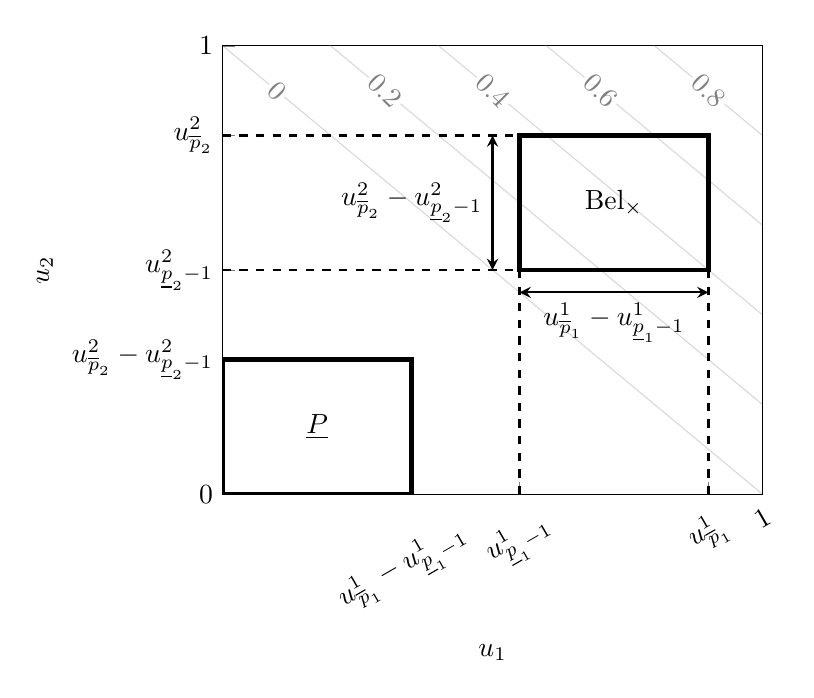
\begin{tikzpicture}
        \begin{axis}[%
            xlabel=$u_1$,
            ylabel=$u_2$,
            xmin=0, xmax=1,
            ymin=0, ymax=1,
            xtick={0.35, 0.55,  0.9, 1},
            xticklabels={$u^1_{\overline{p}_1} - u^1_{\underline{p}_1-1}~~$, $u^1_{\underline{p}_1-1}$, $u^1_{\overline{p}_1}$, $1$},
            ytick={0, 0.3, 0.5,  0.8, 1},
            yticklabels={$0$, $u^2_{\overline{p}_2} - u^2_{\underline{p}_2-1}$, $u^2_{\underline{p}_2-1}$, $u^2_{\overline{p}_2}$, $1$},
            xticklabel style={rotate=30},
            xtick pos=left,
            ytick pos=left,],
            
            \addplot [domain=0:1,samples=40,draw opacity=0.3,color=gray]({x},{1-x});
            \addplot [domain=0:1,samples=40,draw opacity=0.3,color=gray]({x},{1.2-x}); 
            \addplot [domain=0:1,samples=40,draw opacity=0.3,color=gray]({x},{1.4-x}); 
            \addplot [domain=0:1,samples=40,draw opacity=0.3,color=gray]({x},{1.6-x}); 
            \addplot [domain=0:1,samples=40,draw opacity=0.3,color=gray]({x},{1.8-x});

            \node[rotate=-45, fill=white, rounded corners=2pt, inner sep=1pt] (x) at (0.1, 0.9) {\color{gray}0};
            \node[rotate=-45, fill=white, rounded corners=2pt, inner sep=1pt] (x) at (0.3, 0.9) {\color{gray}0.2};
            \node[rotate=-45, fill=white, rounded corners=2pt, inner sep=1pt] (x) at (0.5, 0.9) {\color{gray}0.4};
            \node[rotate=-45, fill=white, rounded corners=2pt, inner sep=1pt] (x) at (0.7, 0.9) {\color{gray}0.6};
            \node[rotate=-45, fill=white, rounded corners=2pt, inner sep=1pt] (x) at (0.9, 0.9) {\color{gray}0.8};
            
            
            \node (a) at (0.9, 0.8) {};
            \node (b) at (0.55, 0.8) {};
            \node (c) at (0.55, 0.5) {};
            \node (d) at (0.9, 0.5) {};
            \draw[ultra thick, black] (c.center) rectangle (a.center) node[pos=0.5]{$\mathrm{Bel}_\times$};
            
            \node (e) at (0, 0.8) {};
            \node (f) at (0, 0.5) {};
            \node (g) at (0.9, 0) {};
            \node (h) at (0.55, 0) {};
            \draw[thick, dashed, black] (e.center) -- (b.center);
            \draw[thick, dashed, black] (f.center) -- (c.center);
            \draw[thick, dashed, black] (g.center) -- (d.center);
            \draw[thick, dashed, black] (h.center) -- (c.center);
            
            \node (i) at (0.35, 0.3) {};
            \node (j) at (0, 0) {};
            \draw[ultra thick, black] (i.center) rectangle (j.center) node[pos=0.5]{$\underline{P}$};
            
            \node (m) at (0.55, 0.45) {};
            \node (n) at (0.9, 0.45) {};
            \node (o) at (0.5, 0.8) {};
            \node (p) at (0.5, 0.5) {};
            \draw [stealth-stealth, thick, black] (m.center) -- (n.center) node[pos=0.5, below]{$u^1_{\overline{p}_1} - u^1_{\underline{p}_1-1}$};
            \draw [stealth-stealth, thick, black] (o.center) -- (p.center) node[pos=0.5, left]{$u^2_{\overline{p}_2} - u^2_{\underline{p}_2-1}$};
        
        \end{axis}
    \end{tikzpicture}
    \caption{Bird view of the \L ukaciewicz 2-copula $C_L$, where the gray lines are the isolines of the copula. $\mathrm{Bel}_\times$ and $\underline{P}$ are represented in the case where the marginals are p-boxes. The thick rectangles represent the bounds on which to compute the H-volume. Numbers $u^i_k$ use the notation of the proof of proposition \ref{prop:convexity_pbox}.}
    \label{fig:copula_convex}
\end{figure}

\subsection{Joining different types of models}
Different models can be used for multiple sources of uncertainty. When some marginals are modeled using possibility distributions and other by p-boxes, it is still possible to derive results similar as those of sections \ref{subsec:necessity_functions} and \ref{subsec:pboxes} if we use natural orders on the marginal focal sets. 
\begin{proposition}
    When joining marginal credal sets induced by a mix of possibility distributions and p-boxes using a copula $C$ the following inclusion hold:
    \begin{itemize}
        \item if $C$ is D-convex, then $\M_{mass}\subseteq \M_{agg}$.
        \item if $C$ is D-concave then $\M_{agg}\subseteq\M_{mass}$ 
    \end{itemize}
\end{proposition}

\begin{proof}
    The proof is similar to the proof of proposition \ref{prop:convexity_pbox} using the fact that for every focal set $a^i_p$ of a possibility distribution, we can still define $\underline{p}_i$ and $\overline{p}_i$ as $\underline{p}_i=1$ and $\overline{p}_i=p$. The rest of the proof is identical.
\end{proof}

\subsection{Other orders}
Instead of considering the natural ordering, or when such an order does not exists, one could consider an arbitrary order between focal sets when defining $\M_{mass}$ as in \eqref{eq:joint_mass}. A few questions arise: is there always an arbitrary order allowing $\M_{robust}\subseteq\M_{mass}$? If such an order exists, is it possible to explicit it in advance, \ie without computing the lower bounds of the credal sets?

It appears that an order allowing $\M_{robust}\subseteq\M_{mass}$ does not always exist. To prove it, let us find an example where no order allows either inclusion.

\begin{example}
Consider the Clayton copula for $\theta=2$ and $n=2$:
\begin{eqnarray*}
    \forall (u_1,u_2)\in\mathbb{R}^2\backslash(0,0), ~C(u_1,u_2)=\frac{u_1u_2}{\sqrt{{u_1}^2+{u_2}^2-{u_2}^2{u_2}^2}}
\end{eqnarray*}
and $C(0,0)=0$ by continuity (we simplified the expression of the copula given in table \ref{tab:familiy_of_copula}). Let us consider $\X_1=\{x^1_1,\, x^1_2,\, x^1_3\}$, $\X_2=\{x^2_1,\, x^2_2,\, x^2_3\}$ and two possibility distributions $\pi_1$, $\pi_2$ over $\X_1$ and $\X_2$ respectively:
\begin{eqnarray*}
    \pi_1(x^1_1)=\pi_2(x^2_1)=0.2 \qquad \pi_1(x^1_2)=\pi_2(x^2_2)=1 \qquad \pi_1(x^1_3)=\pi_2(x^2_3)=0.7 
\end{eqnarray*}
and the marginal credal sets $\M(\pi_1)$, $\M(\pi_2)$ they induce. We note the focal sets as $a^1_1=\{x^1_2\},~a^1_2=\{x^1_2,\, x^1_3\},~a^1_3=\{x^1_1,\,x^1_2,\,x^1_3\}$ and $a^2_1=\{x^2_2\},~a^2_2=\{x^2_2,\, x^2_3\},~a^2_3=\{x^2_1,\, x^2_2,\, x^2_3\}$. By joining $\M(\pi_1)$ and $\M(\pi_2)$ using $C$, we can obtain the lower probability $\low$ of $\M_{robust}$ using equation \eqref{eq:robust_set}, and a total of 6 belief functions $\mathrm{Bel}^{\preceq_1,\preceq_2}_\times$ using equation \eqref{eq:joint_mass} depending on the orders $\preceq_1, \preceq_2$ used to join the marginal masses. For instance if $\preceq_1$ is such that $a^1_3\preceq_1 a^1_1 \preceq_1 a^1_2$ and $\preceq_2$ such that $a^2_1 \preceq_2 a^2_2 \preceq_2 a^2_3$, then the bivariate mass $m_\times$ would be defined as follows:
\begin{eqnarray*}
    m_\times(a^1_3\times a^2_1) &=& C(m_1(a^1_3), m_2(a^2_1))\\
    m_\times(a^1_1\times a^2_1) &=& C(m_1(a^1_3)+m_1(a^1_1), m_2(a^2_1)) - C(m_1(a^1_3), m_2(a^2_1))\\
    m_\times(a^1_3\times a^2_2) &=& C(m_1(a^1_3), m_2(a^2_1) + m_2(a^2_2)) - C(m_2(a^1_3), m_2(a^2_1))\\
    &\dots&
\end{eqnarray*}

If we consider the two events $E_1=\{x^1_2\}\times\{x^2_2,~x^2_3\}$ and $E_2=\{x^1_2,~x^1_3\}\times\{x^2_2\}$, it is possible to show that $\low(E_1)=\low(E_2)\approx0.131$ (by symmetry of the problem) which is obtained for:
\begin{align*}
    &P_1(x^1_1)=0, \qquad&P_1(x^1_2)=0.3, \qquad&P_1(x^1_3)=0.7,\\
    &P_2(x^2_1)=0.2, \qquad&P_2(x^2_2)=0.3, \qquad&P_2(x^2_3)=0.5
\end{align*}
for $E_1$, and similarly with $P_1$ and $P_2$ reversed for $E_2$. Those values were estimated by running simulations, but their exact value can be computed by solving an optimization problem as $C$ is differentiable (although it is a bit tedious to compute). Then for all orders $\preceq_1,~\preceq_2$ on the focal sets of $\pi_1$ and $\pi_2$ it holds:

 \begin{align*}
    \begin{cases}
        \begin{split}
            \mathrm{Bel}_\times^{\preceq_1,\preceq_2}(E_1) \leqslant& \low(E_1)\\
            \mathrm{Bel}_\times^{\preceq_1,\preceq_2}(E_2) >& \low(E_2)
        \end{split}
    \end{cases}
    \qquad\text{ or }\qquad
    \begin{cases}
        \begin{split}
            \mathrm{Bel}_\times^{\preceq_1,\preceq_2}(E_1) >& \low(E_1)\\
            \mathrm{Bel}_\times^{\preceq_1,\preceq_2}(E_2) \leqslant& \low(E_2)
        \end{split}
    \end{cases}
\end{align*}

The table \ref{tab:beliefs_orders} shows a rounded value of $\mathrm{Bel}^{\preceq_1,\preceq_2}_\times$ for all orders for events $E_1$, $E_2$.

\begin{table}[!ht]
\centering
\begin{tabular}{|c||c|c|c|}
\hline
$\mathrm{Bel}^{\preceq_1,\preceq_2}_\times(\mathbf{E_1})$ & $a^2_3\preceq_2a^2_2\preceq_2a^2_1$ & $a^2_3\preceq_2a^2_1\preceq_2a^2_2$ & $a^2_2\preceq_2a^2_3\preceq_2a^2_1$ \\ \hline\hline
$a^1_3\preceq_1a^1_2\preceq_1a^1_1$ & 0.296 & 0.296 & 0.224 \\ \hline
$a^1_3\preceq_1a^1_1\preceq_1a^1_2$ & 0.254 & 0.254 & 0.240 \\ \hline
$a^1_2\preceq_1a^1_3\preceq_1a^1_1$ & 0.296 & 0.296 & 0.224 \\ \hline
$a^1_1\preceq_1a^1_3\preceq_1a^1_2$ & \textbf{0.131} & \textbf{0.131} & 0.279 \\ \hline
$a^1_2\preceq_1a^1_1\preceq_1a^1_3$ & 0.291 & 0.291 & 0.216 \\ \hline
$a^1_1\preceq_1a^1_2\preceq_1a^1_3$ & \textbf{0.131} & \textbf{0.131} & 0.279 \\ \hline
\end{tabular}

\vspace{0.5cm}

\begin{tabular}{|c||c|c|c|}
\hline
$\mathrm{Bel}^{\preceq_1,\preceq_2}_\times(\mathbf{E_1})$ & $a^2_1\preceq_2a^2_3\preceq_2a^2_2$ & $a^2_2\preceq_2a^2_1\preceq_2a^2_3$ & $a^2_1\preceq_2a^2_2\preceq_2a^2_3$ \\ \hline\hline
$a^1_3\preceq_1a^1_2\preceq_1a^1_1$ & 0.259 & 0.180 & 0.180 \\ \hline
$a^1_3\preceq_1a^1_1\preceq_1a^1_2$ & 0.208 & 0.270 & 0.270 \\ \hline
$a^1_2\preceq_1a^1_3\preceq_1a^1_1$ & 0.259 & 0.180 & 0.180 \\ \hline
$a^1_1\preceq_1a^1_3\preceq_1a^1_2$ & 0.251 & 0.293 & 0.293 \\ \hline
$a^1_2\preceq_1a^1_1\preceq_1a^1_3$ & 0.236 & 0.218 & 0.218 \\ \hline
$a^1_1\preceq_1a^1_2\preceq_1a^1_3$ & 0.251 & 0.293 & 0.293 \\ \hline
\end{tabular}

\vspace{1cm}

\begin{tabular}{|c||c|c|c|}
\hline
$\mathrm{Bel}^{\preceq_1,\preceq_2}_\times(\mathbf{E_2})$ & $a^2_3\preceq_2a^2_2\preceq_2a^2_1$ & $a^2_3\preceq_2a^2_1\preceq_2a^2_2$ & $a^2_2\preceq_2a^2_3\preceq_2a^2_1$ \\ \hline\hline
$a^1_3\preceq_2a^1_2\preceq_2a^1_1$ & 0.296 & 0.254 & 0.296 \\ \hline
$a^1_3\preceq_1a^1_1\preceq_1a^1_2$ & 0.296 & 0.254 & 0.296 \\ \hline
$a^1_2\preceq_1a^1_3\preceq_1a^1_1$ & 0.224 & 0.240 & 0.224 \\ \hline
$a^1_1\preceq_1a^1_3\preceq_1a^1_2$ & 0.259 & 0.208 & 0.259 \\ \hline
$a^1_2\preceq_1a^1_1\preceq_1a^1_3$ & 0.180 & 0.270 & 0.180 \\ \hline
$a^1_1\preceq_1a^1_2\preceq_1a^1_3$ & 0.180 & 0.270 & 0.180 \\ \hline
\end{tabular}

\vspace{0.5cm}

\begin{tabular}{|c||c|c|c|}
\hline
$\mathrm{Bel}^{\preceq_1,\preceq_2}_\times(\mathbf{E_2})$ & $a^2_1\preceq_2a^2_3\preceq_2a^2_2$ & $a^2_2\preceq_2a^2_1\preceq_2a^2_3$ & $a^2_1\preceq_2a^2_2\preceq_2a^2_3$ \\ \hline\hline
$a^1_3\preceq_2a^1_2\preceq_2a^1_1$ & \textbf{0.131} & 0.291 & \textbf{0.131} \\ \hline
$a^1_3\preceq_1a^1_1\preceq_1a^1_2$ & \textbf{0.131} & 0.291 & \textbf{0.131} \\ \hline
$a^1_2\preceq_1a^1_3\preceq_1a^1_1$ & 0.279 & 0.216 & 0.279 \\ \hline
$a^1_1\preceq_1a^1_3\preceq_1a^1_2$ & 0.251 & 0.236 & 0.251 \\ \hline
$a^1_2\preceq_1a^1_1\preceq_1a^1_3$ & 0.293 & 0.218 & 0.293 \\ \hline
$a^1_1\preceq_1a^1_2\preceq_1a^1_3$ & 0.293 & 0.218 & 0.293 \\ \hline
\end{tabular}

\caption{Value of $\mathrm{Bel}^{\preceq_1,\preceq_2}_\times$ for $E_1$ and $E_2$ depending on the arbitrary orders $\preceq_1,~\preceq_2$. Values in bald font represent the minimal value attained by the different belief functions, where $\mathrm{Bel}^{\preceq_1,\preceq_2}_\times(E)=\low(E)$.}
\label{tab:beliefs_orders}
\end{table}

Answering the question ``if an order allowing $\M_{robust}\subseteq\M_{mass}$ exists, is it possible to explicit it in advance?'' is not as trivial. Indeed the order will be dependent of the copula. We ran simulations where we created different possibility distributions (for $card(\X_1)=card(\X_2)\in\{3,4\}$), sampled the marginal credal sets and joined them with a copula $C$ to get $\inf\M_{robust}$ and compared its values with the one of $\mathrm{Bel}^{\preceq_1,\preceq_2}$.
\begin{itemize}
	\item When running the simulation with the lower Fréchet–Hoeffding copula $C(u,v)=\max(0,u+v-1)$, we observe that a specific couple of order always works: $\preceq_1:~a^1_3\preceq_1a^1_2\preceq_1a^1_1$ and $\preceq_2~a^2_3\preceq_2a^2_2\preceq_2a^2_1$, while other orders do not permit the inclusion $\M_{robust}\subseteq\M_{mass}$ all the time.
\end{itemize}
The order is thus copula dependent.

We ran simulation for the lower and upper Fréchet-Hoeffding copulas, as well as with the copulas presented in table \ref{tab:familiy_of_copula}. We were only able to find examples where no orders were working for the Ali-Mikail-Haq copula with $\theta>0$, for the Gumbel copula and for Clayton copulas. 
\end{example}

\pagebreak